\chapter{Estudos de Caso}
\label{cap:estudos-de-caso}

%Explicar o porque de cada cenário
%Detalhar implementação e experimentos realizados:

Com o intuito de validar a arquitetura proposta foram realizados dois estudos de caso envolvendo diferentes cenários de Cidades Inteligentes em um ambiente simulado de experimentação.
Priorizamos implementar cenários de experimentação onde pudéssemos explorar todos os requisitos apresentados no Capítulo \ref{cap:proposta}.
Através desses dois experimentos, pudemos validar a solução apresentada para construção de um ambiente simulado de experimentação para plataformas de Cidades Inteligentes.
Foi possível exercitar as principais funcionalidades necessárias para a realização de experimentos desse tipo, através da integração do InterSCSimulator e a plataforma InterSCity.

No primeiro cenário, realizamos experimentos no contexto de estacionamento inteligente (conhecido com \textit{Smart Parking}), onde carros circulam pela cidade e, ao
final do seu percurso, procuram por uma vaga de estacionamento disponível mais próxima do seu destino, utilizando-se da plataforma para isso.
Nesse cenário, incluímos um novo agente à simulação e implementamos um mecanismo para publicação dos eventos ocorridos e requisição a serviços da plataforma em tempo real
e de forma assíncrona.

O segundo cenário de experimentação envolve o tráfego de carros inteligente através da utilização de Placas de Mensagens Variadas (PMVs) espalhadas pela cidade.
Nesse cenário, a plataforma identifica trechos de maior trânsito e atua na cidade atualizando as mensagens apresentadas pelas PMVs em tempo real, notificando os
motoristas da lentidão no trecho, que por sua vez podem recalcular a sua rota evitando congestionamentos.
Para viabilizar esse experimento fizemos uso das melhorias implementadas no primeiro cenário acrescidas de outras tais como: modificação do modelo de trânsito para melhor se adequar a realidade e
implementação do mecanismo de recebimento de comandos de atuação em tempo de execução.

A seguir a arquitetura do simulador InterSCSimulator e da plataforma InterSCity serão apresentadas, haja vista que essas foram as ferramentas utilizadas para o desenvolvimento
dos estudos de caso.
Além disso, cada um dos cenários de Cidades Inteligentes mencionados serão apresentados detalhadamente, visando exemplificar a implementação da arquitetura proposta e os resultados experimentais obtidos.
Ao final, realizaremos uma análise crítica sobre os resultados obtidos, apontando possíveis melhorias a serem feitas.

\section{Ferramentas}

O simulador InterSCSimulator e a plataforma InterSCity serão detalhados quanto as suas respectivas arquiteturas.
Faremos uma discussão de como os \textbf{requisitos fundamentais e de integração} apresentados no Capítulo \ref{cap:proposta} serão atendidos em cada ferramenta.

\subsection{InterSCSimulator}

O InterSCSimulator é um simulador de código aberto baseado em agentes para Cidades Inteligentes que oferece uma interface simples para definição de
cenários de larga escala \citep{santana_17}.
Pelo fato de ser possível configurar o tempo que dura um ciclo de simulação na ferramenta, ela já atende um dos \textbf{requisitos fundamentais} descritos na Seção \ref{sec:requisitos}.
Com isso, podemos dizer que um ciclo de simulação é igual a um segundo real.
É sabido que é necessário termos uma execução com noção de tempo real (um segundo de simulação igual a aproximadamente um segundo real) e permitir a
interferência em tempo de execução por terceiros para a construção desse ambiente integrado de experimentação.

Para atingir a escalabilidade mencionada, o InterSCSimulator foi implementado usando a linguagem \textit{Erlang}.
Essa é uma linguagem funcional que visa facilitar a implementação de aplicações de larga escala, paralelas e distribuídas.
Algumas características herdadas do modelo de atores, que é implementado pelo \textit{Erlang}, são: paralelismo, execução distribuída, tolerância a falhas e
protocolo de comunicação \citep{santana_17}.
Essa escalabilidade é importante para que possamos atender o \textbf{requisito fundamental} que diz respeito à capacidade de geração de grande massa de dados
para a plataforma.
O InterSCSimulator é capaz de simular cenários com milhões de agentes executando simultaneamente, possibilitando trabalhar-se em uma escala realista para cidades de grande porte.

O InterSCSimulator foi implementado por Eduardo Zambom Santana, doutorando do nosso grupo de pesquisa, baseado no simulador de âmbito geral \textit{Sim-Diasca}.
A Figura \ref{fig:simulator_architecture} representa a sua arquitetura da seguinte forma: em azul estão os diferentes tipos de agentes que podem existir no ambiente
simulado e, em vermelho a definição dos cenários de Cidades Inteligentes.
Tudo isso sendo executado no topo do simulador \textit{Sim-Diasca}.

\begin{figure}[ht]
	\centering
	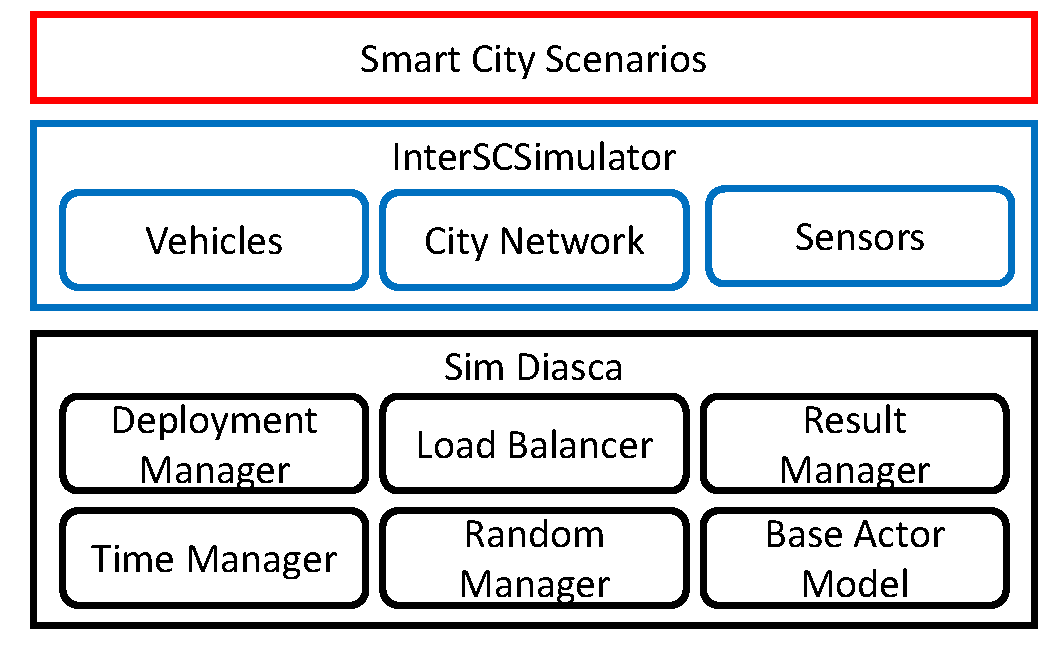
\includegraphics[width=0.5\textwidth]{figuras/Arquitetura.pdf}
	\caption{Arquitetura do InterSCSimulator}
	\label{fig:simulator_architecture}
\end{figure}

Fazendo um paralelo com um dos \textbf{requisitos de integração}, cada \textit{Recurso} da cidade pode ser modelado como um agente da simulação, ou seja, um carro, uma vaga de estacionamento ou um ponto
de parada de ônibus serão representados como agentes (caixas azuis na Figura \ref{fig:simulator_architecture}).
Na definição desses agentes especificamos o seu comportamento a cada passo da simulação.
Com isso, podemos descrever quais as \textit{Capacidades} de cada agente e adotar modelos compatíveis com a realidade das cidades modernas.
Por exemplo, podemos determinar que um agente do tipo carro envie sua localização a cada passo da simulação e que ele recalcule a sua rota apenas quando deparado com uma PMV.
O interessante dessa arquitetura baseada em agentes é o fato da sua implementação ter um alto grau de independência, onde é preciso apenas a definição das mensagens que serão trocadas em tempo
de execução.

No contexto desta dissertação, foi adicionado um novo elemento à arquitetura da ferramenta para troca de dados com sistemas externos em tempo de execução,
sendo esse um dos \textbf{requisitos fundamentais e de integração} para obtermos um ambiente realista de experimentação.
Esse novo elemento nada mais é do que um novo agente, cujo papel é receber e enviar mensagens de sensores e atuadores, seja no contexto de outros agentes ou de outros sistemas.

Na implementação de um agente do InterSCSimulator, podemos definir diversos comportamentos em diferentes momentos do seu cliclo de vida.
É possível especificar o que será feito durante a sua criação, a sua destruição, a sua primeira ação na simulação e durante cada ciclo de execução.
Com isso, condições e caminhos dependentes do estado da simulação podem ser definidos para cada um dos tipos de agentes, flexibilizando a implementação dos
mais diversos modelos e formas de prover suas capacidades.
Essa liberdade para implementação de diversos comportamentos dos agentes nos permite usar modelos realistas e viabilizar as capacidades dos recursos no contexto das cidades,
atendendo aos \textbf{requisitos fundamentais e de integração}.
Por exemplo, um carro, após a sua partida em direção ao seu destino, calcula a cada ciclo de execução o fluxo de carros na via em que se encontra para o cálculo da
sua velocidade naquele instante, além de publicar a sua posição atual.
Nesse caso, podemos utilizar os mais diversos modelos matemáticos para calcular o fluxo de carros ou para determinar a sua velocidade, ao passo que a sua capacidade
de publicar sua localização georreferenciada também é atendida.

Na Figura \ref{fig:simulator_components}, são apresentados os componentes do simulador.
Inicialmente são dadas entradas para a simulação (arquivos XML) que em conjunto formam o cenário a ser simulado.
Esse cenário é executado e a saída é criada com todos os eventos ocorridos na simulação.
A partir dessa saída, existe a possibilidade de geração de uma visualização em um mapa ou através de gráficos.

\begin{figure}[ht]
	\centering
	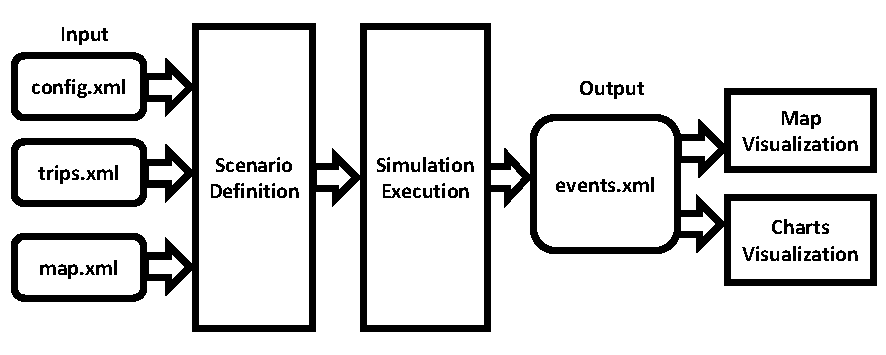
\includegraphics[width=0.7\textwidth]{figuras/Components.pdf}
	\caption{Componentes do InterSCSimulator}
	\label{fig:simulator_components}
\end{figure}

Como entrada, o InterSCSimulator recebe três arquivos XML.
O \textit{config.xml} contém parâmetros da simulação: o tempo total, o formato do
arquivo de saída e o caminho para o diretório contendo os outros arquivos de entrada e para geração do arquivo de saída.
O grafo representando a infraestrutura rodoviária da cidade é descrito no arquivo \textit{map.xml}: as vias são representadas pelas arestas e as esquinas entre
duas ou mais vias pelos nós.
Por fim, as viagens a serem executadas são especificadas no arquivo \textit{trips.xml}, cada viagem contendo o seu tempo de início, modo de transporte, origem e destino.
Todas as ações realizadas pelos agentes são salvas no arquivo \textit{output.xml}, podendo haver quatro ações possíveis: 1) início de viagem, 2) saída de uma via,
3) entrada em uma via, e 4) chegada ao destino final.
O tempo, a localização e o modo de transporte utilizado pelo agente são registrados quando essas ações são salvas.

Os modos de transportes suportados até o momento são: carro, ônibus, metrô e a pé.
Neste trabalho, além de melhorias feitas nos modelos existentes, novos agentes foram adicionados ao simulador, além da nova possibilidade de publicação e o recebimento de
eventos em tempo de execução de maneira assíncrona.

\subsection{Plataforma InterSCity}
\label{sec:interscity}

A plataforma InterSCity é um projeto de código aberto, baseado em microsserviços que visa permitir a pesquisa colaborativa, desenvolvimento e experimentos em Cidades
Inteligentes~\citep{arthur_17}.
A plataforma foi desenvolvida baseada em uma arquitetura de referência para plataformas de Cidades Inteligentes~\citep{santana_2016}, ela provê um conjunto de serviços de
alto-nível baseado em nuvem para gerenciar recursos de IoT heterogêneos.

O InterSCity visa solucionar dois dos principais problemas arquiteturais no desenvolvimento de uma plataforma de alta qualidade que possa ser usada na prática, no
contexto de Cidades Inteligentes: escalabilidade e evolução do software~\citep{arthur_17}.
Escalabilidade é necessária pelo fato da plataforma ter que interagir com um grande número de dispositivos IoT espalhados pela cidade, milhões de usuários e
um grande tráfego de dados.
Como as cidades mudam constantemente, a questão da evolução é essencial, já que requisitos podem surgir e/ou mudar a qualquer momento.
Adaptar a plataforma para modificar e/ou incorporar novas funcionalidades, não deve ser um empecilho.
Para resolver esses dois problemas apresentados, foram adotadas as seguintes estratégias:

\begin{itemize}
	\item Modularidade via microsserviços
	\item Modelos e dados distribuídos
	\item Evolução descentralizada
	\item Reúso de projetos de software livre
	\item Adoção de padrões abertos
	\item Comunicação síncrona e assíncrona
	\item Serviços livres de estado
\end{itemize}

A Figura \ref{fig:platform_architecture} apresenta a arquitetura da plataforma InterSCSity.
Atualmente, ela é composta de 7 microsserviços:
\textit{Resource Adaptor}, oferece uma abstração para comunicação com os dispositivos IoT;
\textit{Data Collector}, responsável por coletar os dados dos sensores conectados;
\textit{Actuator Controller}, oferece uma interface para atuação junto aos dispositivos de IoT com tal capacidade;
\textit{Resource Catalog}, possui dados estáticos dos recursos da cidade cadastrados;
\textit{Resource Discovery}, provê um serviço de descoberta de recursos;
\textit{Data Processor}, oferece um serviço de processamento de dados em tempo real e histórico;
e \textit{Resource Viewer}, disponibiliza uma visualização simples dos recursos da cidade. 

\begin{figure}[ht]
	\centering
	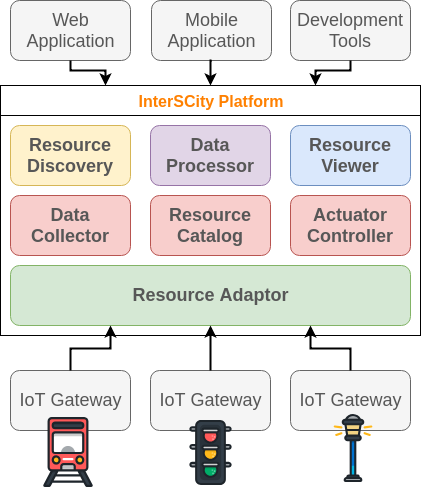
\includegraphics[width=0.5\textwidth]{figuras/platform_architecture.png}
	\caption{Arquitetura da plataforma InterSCity}
	\label{fig:platform_architecture}
\end{figure}

A comunicação entre esses microsserviços pode se dar de maneira síncrona ou assíncrona, dependendo da situação.
A comunicação síncrona é feita via API \textit{Restful}, ou seja, requisições HTTP; e a assíncrona se dá via RabbitMQ\footnote{https://www.rabbitmq.com/}, uma implementação do protocolo AMQP.
O objetivo do protocolo AMQP é criar um padrão aberto para troca de mensagens assíncronas interoperável e de larga escala~\citep{vinoski_2006}.
A principal vantagem desse protocolo é permitir que o \textit{broker} de mensagens tome as decisões de roteamento, não necessitando a aplicação ter conhecimento
desse processo~\citep{vinoski_2006}.

A plataforma traz uma abstração chamada \textit{Resource}, que representa um recurso real da cidade, como ônibus, hospital, paradas de ônibus.
Cada um desses \textit{Resources} possuem \textit{Capabilities}, que podem ser de sensoriamento ou atuação, usualmente vinculados a algum tipo de dispositivo de IoT,
como capacidade de medir temperatura ou capacidade de mudar o estado de um semáforo.
Esses conceitos são os mesmos apresentados na Seção \ref{sec:requisitos}, como requisitos para a construção de um ambiente integrado de experimentação para Cidades Inteligentes.
Como apresentado na seção anterior, semanticamente, esses recursos e capacidades aqui apresentados estarão associados a agentes e à definição de ações durante o seu
ciclo de vida no InterSCSimulator.

Nas seções a seguir, serão apresentados os dois estudos de caso envolvendo estacionamento e tráfego de carros inteligente que fizeram uso do InterSCSimulator e da plataforma InterSCity
para Cidades Inteligentes.

\section{Estacionamento Inteligente}

Neste estudo de caso, simulamos motoristas realizando seus respectivos percursos de carro e ao final procurando uma vaga disponível mais próxima ao
seu destino, provavelmente utilizando um aplicativo móvel que se comunica com a plataforma InterSCity.
Esse tipo de aplicativo poderia evitar alguns transtornos para os motoristas na árdua missão de estacionar seus carros no centro das grandes metrópoles.

A implementação deste cenário seguindo a arquitetura proposta no Capítulo \ref{cap:proposta}, bem como o experimento realizado, serão discutidos nas seções seguintes.

\subsection{Implementação}
\label{sec:smart_parking}

Ao resgatar os conceitos de recursos da cidade e capacidades para este cenário, temos os carros e as vagas de estacionamento sendo recursos, onde os carros são capazes de
fornecer a sua geolocalização (por exemplo, via GPS) e as vagas de fornecer informação quanto à sua disponibilidade (por exemplo, através de sensores infravermelhos e uma
rede de sensores).

Este cenário foi definido com o intuito de realizar experimentos envolvendo o serviço de descoberta de recursos da plataforma InterSCity.
Portanto, o aplicativo enviaria a posição do carro naquele momento, o seu destino final e o raio de busca, e a plataforma traria uma lista de vagas de estacionamento
disponíveis nas proximidades.
Já no InterSCSimulator, foi necessário realizar algumas melhorias para que os \textbf{requisitos fundamentais} fossem atendidos.
Um novo agente para gerenciar as vagas de estacionamento da cidade, chamado \textit{Parking Controller}, foi implementado.
Esse agente possui a responsabilidade de gerenciar e armazenar dados referentes às vagas de estacionamento e fazer a interface de comunicação com o componente de
integração que será apresentado mais adiante.
Além disso, modificamos o modelo de viagem do agente do tipo carro.
Anteriormente, o \textit{Carro} saia de uma origem e percorria o seu trajeto até o destino, agora, ao chegar próximo do seu destino, ele requisita uma vaga disponível mais
próxima e se dirige até ela.
Com essas melhorias, pudemos simular um cenário que se aproxima da realidade.

Para ilustrar o modelo descrito, apresentamos o ciclo de execução de um agente carro neste cenário:

\begin{enumerate}
    \item O agente \textit{Carro} é criado

    \item O caminho mais curto entre a origem e o destino é calculado

    \item O agente parte da sua origem no tempo determinado

    \item Ao chegar no nó anterior ao seu destino, uma vaga de estacionamento disponível é requisitada ao agente \textit{Parking Controller}

    \item Ao receber a vaga de estacionamento, o seu trajeto é recalculado em direção a ela

    \item O agente se direciona e estaciona na vaga descoberta 
\end{enumerate}

Um fluxo alternativo a essa execução seria o carro modificar o seu percurso em direção à vaga de estacionamento (disponível até então), e ao chegar a ela outro
carro a ter ocupado antes, sendo esse um caso comum nas grandes cidades.
Nesse caso, outra vaga de estacionamento é requisitada aumentando o seu raio de busca com o intuito de sempre encontrar vagas disponíveis.
Caso o agente do tipo carro necessitar realizar mais de três buscas de vagas disponíveis, o mesmo encerra a sua execução.

Quando o agente \textit{Carro} por fim estaciona em uma vaga disponível, o agente \textit{Parking Controller} é notificado e atualiza a sua estrutura de dados indicando
que a vaga foi ocupada pelo carro.
Esse agente é responsável também por atualizar o estado da vaga de estacionamento na plataforma.

Agora pensando nos \textbf{requisitos de integração}, o simulador precisa requisitar a plataforma em busca de vagas disponíveis mais próximas e atualizar o estado
das vagas de estacionamento.
A plataforma InterSCity provê uma API \textit{Restful} para comunicação com seus serviços (como o de descoberta de recursos), e o estado dos seus recursos podem ser
atualizados através da própria API ou via protocolo AMQP (\textit{Advanced Message Queuing Protocol}).
Esse levantamento é importante para a tomada de decisão de quais as responsabilidades e como será implementado o componente de integração.
Tendo em vista que a complexidade do componente de integração deve ser a menor possível, e a não existência de um meio de publicação de eventos em tempo de execução
no InterSCSimulator, decidimos utilizar o RabbitMQ (implementação do protocolo AMQP) na implementação desse novo meio de comunicação.
Com isso, o simulador pode atualizar o estado das vagas diretamente na plataforma de forma assíncrona, sem necessidade de auxílio do componente de integração.
As requisições HTTP feitas ao serviço de descoberta da plataforma forma realizadas pelo componente de integração, principalmente pelo fato de requisições HTTP serem
síncronas, o que poderia travar a simulação na espera por uma resposta.

Para facilitar o entendimento da integração realizada, dividiremos a explicação em duas partes: a primeira visando a requisição de vagas disponíveis mais próximas
do carro ao serviço de descoberta da plataforma InterSCity; e a segunda apresentando o fluxo de atualização do estado de uma vaga de estacionamento (ocupada
ou disponível) baseada na simulação.

A Figura \ref{fig:descoberta} apresenta a integração realizada para utilização do serviço de descoberta provido pela plataforma InterSCity.
O componente de integração foi chamado de \textit{Parking Spot Discoverer}, e foi implementado como um agente Erlang que consegue se comunicar com os agentes da
simulação via troca de mensagens.
O uso do componente de integração se fez necessário para que a simulação exerça a carga que aplicações exerceriam utilizando o protocolo HTTP para acessar
a API \textit{Restful}.
Como dito, requisições HTTP são síncronas, e sua realização dentro da simulação atrasaria consideravelmente a sua finalização, já que bloquearia a
execução dos agentes enquanto aguardariam a resposta da plataforma.
Antes de chegarmos a tal solução, implementamos uma versão onde o próprio simulador realizava requisições HTTP para a plataforma em tempo de execução, entretanto,
essa solução gerou um enorme gargalo.
Descrevemos abaixo o fluxo de atividades apresentado na Figura \ref{fig:descoberta}.

\begin{enumerate}
    \item Ao chegar a um nó, antes do seu destino, o \textit{Car} solicita a vaga de estacionamento para o agente \textit{Parking Controller}, passando a sua
	localização como parâmetro.

	\item O agente \textit{Parking Controller} envia a localização para o \textit{Parking Spot Discoverer} que solicita a vaga disponível mais próxima,
	em um raio de 500 metros.

	\item O \textit{Parking Spot Discoverer} faz uma requisição HTTP para o serviço de descoberta da plataforma que retorna a vaga em questão.
	Caso não seja encontrada uma vaga disponível (não ocupada) em um raio de 500 metros, esse raio é multiplicado por dois até que se encontre uma vaga
	disponível.

	\item O identificador da vaga é retornado para o agente \textit{Parking Controller} e ele marca a vaga como utilizada em uma estrutura de dados mantida no simulador.

    \item O identificador da vaga é recebido pelo agente \textit{Car} e a rota é recalculada para chegar até ela.
\end{enumerate}

\begin{figure}[ht]
	\centering
	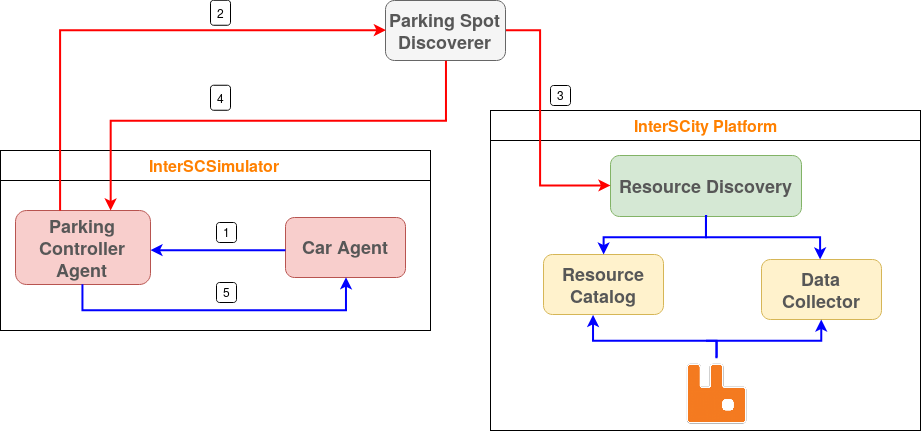
\includegraphics[width=\textwidth]{figuras/integration_get_data_smart_parking.png}
	\caption{Integração para descoberta de vagas livres próximo do destino da
	viagem}
	\label{fig:descoberta}
\end{figure}

A Figura \ref{fig:atualizacao} apresenta a integração realizada com o intuito de atualizar o estado das vagas de estacionamento na plataforma baseado nos
acontecimentos da simulação.
Como foi adicionado a funcionalidade de publicação dos eventos da simulação via RabbitMQ para os interessados, não foi necesário a utilização do
componente de integração, já que a plataforma também utiliza o mesmo protocolo para divulgação dos seus dados entre os microsserviços.
O fluxo apresentado na Figura \ref{fig:atualizacao} contém os seguintes passos.

\begin{enumerate}
    \item O agente \textit{Car} estaciona na vaga do estacionamento e notifica o \textit{Parking Controller}.

	\item O \textit{Parking Controller} informa, via \textit{RabbitMQ}, que a vaga está ocupada usando o seu identificador.

	\item O \textit{RabbitMQ} repassa esse dado para os microsserviços \textit{Resource Catalog} e \textit{Data Collector}.
\end{enumerate}

\begin{figure}[ht]
	\centering
	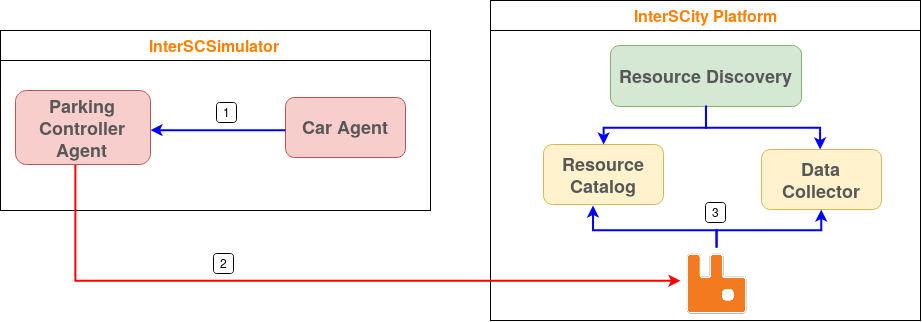
\includegraphics[width=\textwidth]{figuras/integration_publish_data_smart_parking.png}
	\caption{Integração para publicar dados}
	\label{fig:atualizacao}
\end{figure}

Vale ressaltar que as atividades 2 e 3 apresentadas na Figura \ref{fig:atualizacao} também são executadas quando a vaga é liberada.
Após dez minutos que o agente está estacionado na vaga, o agente \textit{Parking Controller} libera a vaga na estrutura de dados mantida dentro do simulador e informa o
ocorrido para a plataforma.
Com isso, a plataforma atualiza os dados da vaga quando ela é ocupada e quando liberada.

Após a implementação da arquitetura descrita, fomos capazes de executar experimentos de larga escala no contexto de estacionamento inteligente.
Os resultados obtidos serão apresentados na próxima seção.

\subsection{Experimento}
\label{sec:exp_smart_parking}

Neste experimento, tentamos verificar a escalabilidade dos microsserviços envolvidos da plataforma InterSCity, para isso utilizamos dados reais de uma das maiores metrópoles do mundo: São Paulo.
Dados abertos da cidade de São Paulo foram utilizados para a definição do cenário de simulação do ambiente integrado.
Utilizamos dados extraídos da pesquida OD (Origem-Destino) realizada pela Companhia de Metrô da cidade de São Paulo e do OpenStreet Maps para a definição de cenário.
A seguir, esses dados, bem como suas fontes, utilizados na configuração do experimento serão detalhados:

\begin{itemize}
    \item \textbf{Pesquisa Origem-Destino (OD)}: criamos as viagens de carro simuladas com base na pesquisa OD realizada pela Companhia de Metrô de São Paulo em 2007.
        \footnote{Pesquisa Origem-Destino - https://transparencia.metrosp.com.br/dataset/pesquisa-origem-e-destino/resource/dd9382bf-fbbe-4ca4-bd32-bf6150a59c4b}
        Essa pesquisa descreve as viagens de 200.000 pessoas e extrapola os dados para toda a população da cidade.
        A pesquisa inclui informações sobre a origem, o destino, o modo de transporte e a hora de partida.
        Esses dados foram utilizados para definir o comportamento dos agentes do tipo carro na simulação.
        Para gerar a carga de trabalho para a plataforma, simulamos o tráfego em São Paulo durante um dos horários de pico, das 5h40 às 8h40.
        Na pesquisa OD, há 492.976 carros que começam suas viagens durante o intervalo de tempo considerado.

    \item \textbf{OpenStreet Maps}: para criar o grafo viário da cidade de São Paulo usado na simulação, usamos o mapa do OpenStreet Maps.
        Esse mapa contém todas as ruas e junções da cidade, em conjunto com um vasto número de atributos, como comprimento, capacidade e velocidade limite.
        Tais informações são usadas pelo simulador para definir as rotas percorridas pelos carros durante a realização de suas viagens, bem como simular o impacto do tráfego na velocidade dos carros.

    \item \textbf{Vagas de Estacionamento}: criamos as vagas de estacionamento na simulação baseado nos dados obtidos através do OpenStreet Maps e do Zona Azul
        \footnote{http://www.cetsp.com.br/consultas/zona-azul/mapa-zona-azul/mapa-zona-azul.aspx}
        (serviço de estacionamento rotativo da cidade de São Paulo).
        Informações de 467.741 vagas de estacionamento foram coletadas, elas foram derivadas a partir de dados de estacionamentos obtidos através do OpenStreet Maps, onde é possível obter
        a capacidade máxima (número de carros), e de vagas individuais do Zona Azul.
\end{itemize}

Nas Figuras \ref{fig:map-spots-distribution} e \ref{fig:map-destinations-distribution}, são apresentadas as distribuições das vagas de estacionamento e destinos de viagens de carros, respectivamente,
utilizadas nesse experimento.
Os destinos apresentados na Figura \ref{fig:map-destinations-distribution}, são referentes a todas as viagens realizadas no decorrer de toda a simulação.
É importante notar que a distribuição das vagas de estacionamento baseada nesses dados reais está mais concentrada no centro da cidade do que os destinos das viagens.
Isso pode levar a situaçãoes onde o agente do tipo carro pode realizar mais de três tentativas de busca de vagas disponíveis e ainda sim não conseguir estacionar.
Nesse caso, o usuário do aplicativo pararia de utilizá-lo e o agente do tipo carro terminaria sua execução, como apresentado na Seção \ref{sec:smart_parking}.

\begin{figure}[!ht]
    \centering
    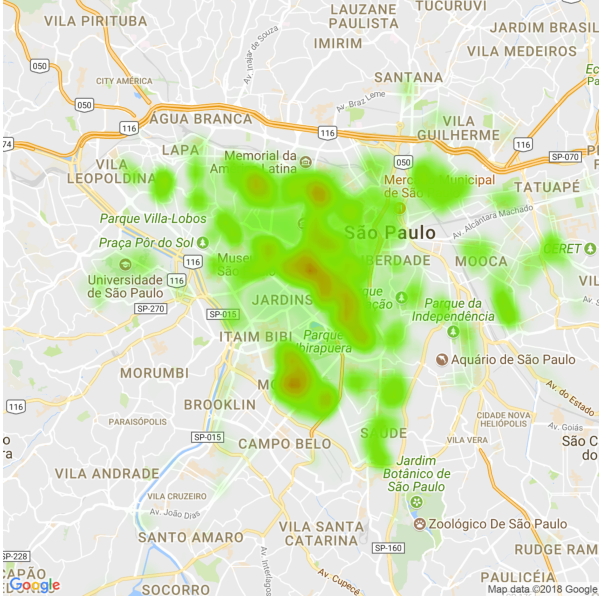
\includegraphics[width=8cm]{figuras/mapa_vagas.pdf}
    \caption{Mapa de calor com a distribuição das vagas de estacionamento utilizadas no experimento.}
    \label{fig:map-spots-distribution}
\end{figure}

\begin{figure}[!ht]
    \centering
    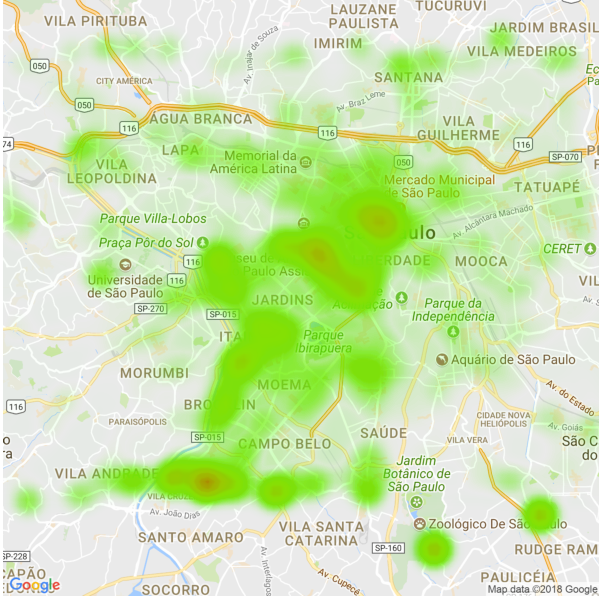
\includegraphics[width=8cm]{figuras/mapa_viagens.pdf}
    \caption{Mapa de calor com a distribuição dos destinos de viagens de carro utilizadas no experimento.}
    \label{fig:map-destinations-distribution}
\end{figure}

Os passos a seguir foram executados no decorrer desse experimento:

\begin{enumerate}
    \item Execução de uma instância em modo de produção da plataforma InterSCity em um ambiente de nuvem. Esse ambiente proporciona maior flexibilidade para variação do número de microsserviços em tempo
        de execução.

    \item Habilitação do mecanismo de elasticidade automática (\textit{auto-scaling}) para os microsserviços da plataforma baseado na variação de carga de trabalho.

    \item Configuração do simulador em um ambiente isolado da plataforma. Assim, o gasto de recursos computacionais do simulador não interfere no uso da plataforma.

    \item Realização da simulação do cenário de estacionamento inteligente.

    \item Monitoramento do desempenho e o uso de recursos da plataforma durante toda a simulação.

    \item Analize os resultados obtidos.
\end{enumerate}

Inicialmente, foi necessária a configuração de ambas as ferramentas em conjunto com seu componente de integração em um ambiente de nuvem.
Os microsserviços da plataforma InterSCity, o simulador InterSCSimulator e ferramentas auxiliares foram implantados na forma de contêineres Docker \footnote{https://www.docker.com/}.
Utilizamos a infraestrutura provida pelo Google Cloud Platform (GCP) \footnote{https://cloud.google.com/} para a realização do experimento, sendo esse o ambiente ideal para a execução da plataforma
InteSCity, como visto na Seção \ref{sec:interscity}.
No contexto do GCP, fizemos bastante uso do Google Kubernetes Engine (GKE), sendo esse um serviço que provê um ambiente gerenciado e de produção para implantação de contêineres de
aplicações.
O Kubernetes foi utilizado principalemte para automatizar a reinicialização, a replicação e dimensionamento do número de contêineres.
Além disso, o kubernetes traz uma vantagem para a reprodutibilidade do experimento que é a especificação da infraestrutura como código, garantindo a correta aplicação das regras de implantação.
Todo o código fonte utilizado para a realização desse experimento está disponível como software livre na web \footnote{https://github.com/LSS-USP/interscity-k8s-experiment}.

Nós dividimos o \textit{cluster} utilizado em cinco diferentes \textit{pools} de máquinas virtuais para que o Kubernetes pudesse gerenciar os contêineres no contexto apropriado.
Na Figura \ref{fig:node-pools}, são apresentados os \textit{pools} de nós, contendo o número e o tipo de máquinas virtuais utilizadas por cada um no GCP
\footnote{https://cloud.google.com/compute/docs/machine-types}.
O \textit{pool} da plataforma possui 25 máquinas do tipo n1-standard-2 (2 CPUs virtuais e 7.5GB memória) e executa os microsserviços da plataforma InterSCity.
Existem três conjuntos de nós adicionais (representados em azul) compostos por n1-high-2 máquinas (2 CPUs virtuais e 13GB de memória), que executam os serviços de suporte da plataforma InterSCity.
Ambos MongoDB e PostgreSQL têm 5 nós sendo executados de maneira distribuída, instâncias tolerantes a falha de seus respectivos sistemas de banco de dados.
O RabbitMQ possui uma máquina dedicada em um \textit{pool} isolado.
MongoDB é implementado usando a estratégia de conjunto de réplicas (\textit{replica set}), onde operações de leitura são distribuídas entre nós secundários (escravos), e operações de escrita são
sempre executadas no nó primário (mestre).
A mesma estratégia é adotada na implantação do PostgreSQL, para otimizar as operações de leitura executadas pelo \textit{Resource Catalog}.
Finalmente, o InterSCSimulator é executado em sua própria máquina n1-highmem-16 (16 CPUs virtuais e 104 GB de memória), isoladas do resto do serviços.

\begin{figure}[ht]
	\centering
	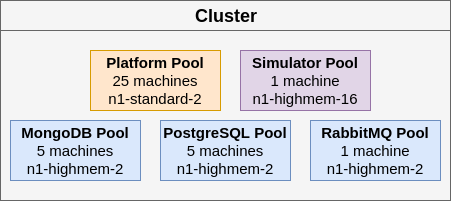
\includegraphics[width=0.7\textwidth]{figuras/node-pools.png}
    \caption{Configuração do \textit{cluster} para o experimento.}
	\label{fig:node-pools}
\end{figure}


Para o conjunto de nós da plataforma, o Kubernetes pode programar a implantação de vários contêineres para a mesma máquina, dependendo da disponibilidade de recursos computacionais.
A distribuição de contêineres nos 25 nós pode diferir de uma rodada do experimento para a outra, e é uma variável que não controlamos durante o experimento.
Para avaliar o impacto de tais variações na análise, realizamos 15 rodadas desse experimento e verificamos a variabilidade dos resultados.

Como estávamos interessados em avaliar a escalabilidade da plataforma considerando um cenário de Cidades Inteligentes com uma carga de trabalho variável, usamos dimensionamento automático
(\textit{auto-scaling}) para o \textit{Resource Catalog}, \textit{Resource Discovery}, \textit{Data Collector}, já que eles são projetados para escalar horizontalmente.
Para esse propósito, especificamos um valor alvo de 60\% de uso da CPU para cada um desses serviços, permitindo que o sistema aumente ou diminua o número de contêineres por serviço baseado nisso.
O sistema balanceia a carga de trabalho para corresponder ao valor alvo de uso da CPU, considerando o uso médio da CPU dos contêineres em execução, que é medido a cada 30 segundos.
Inicialmente, cada serviço tem quatro contêineres, que é definido como o número mínimo de contêineres em execução.
Esse número pode aumentar à medida que os recursos computacionais ficarem disponíveis no \textit{pool} de nós da plataforma.
Os contêineres são executados por trás de um serviço de balanceamento de carga.

Embora possamos nos beneficiar das propriedades de elasticidade do GCP, adicionando e removendo automaticamente nós ao \textit{cluster} através da sua funcionalidade de dimensionamento automático,
isso introduziria outro nível de incerteza em nosso experimento, já que, na nossa experiência, o tempo levado para criar novas máquinas virtuais pode variar consideravelmente.
Sabendo disso, criamos todos os nós previamente, antes de iniciar o experimento, mantendo-os em execução ao longo de todo experimento.

Como dito anteriormente, executamos 15 rodadas de experimentos, onde cada uma durou 3h, correspondendo ao horário de pico da manhã da cidade de São Paulo descrito no início desta seção.
Na Figura \ref{fig:workload}, podemos ver a carga de trabalho média gerada pela simulação durante todo o experimento e o seu desvio padrão (linhas pretas no topo de cada barra).
Vale notar que nos primeiros 80 minutos de simulação, temos um crescimento constante da carga de trabalho.
No intervalo aproximado de uma hora, entre 60 e 120 minutos, observamos o período de maior carga do experimento, considerando que o pico máximo de requisições ocorre após 80 minutos, correspondendo a mais
de 113.000 requisições em 10 minutos.
No total, mais de um milhão de requisições foram realizadas para a plataforma durante o tempo de experimento.
Considerando que para responder cada uma dessas requisições requer um conjunto complexo de operações com várias etapas internas, isso se traduz em uma carga computacional muito alta.

\begin{figure}[ht]
	\centering
	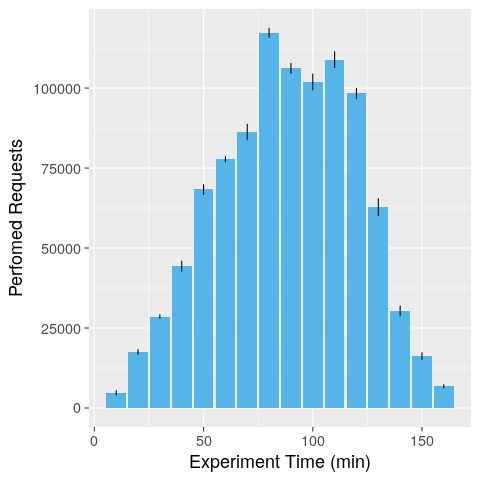
\includegraphics[width=0.7\textwidth]{figuras/workload.png}
    \caption{Média da carga de trabalho gerada pelo InterSCSimulator no decorrer do experimento.}
	\label{fig:workload}
\end{figure}

A Figura \ref{fig:auto-scaling} mostra a criação e destruição dinâmica de contêineres da plataforma InterSCity devido à aplicação da estratégia de dimensionamento automático em uma única rodada
do experimento.
A replicação inicial das instâncias de Kong (balaceador de carga) foi suficiente para suportar toda a carga de trabalho durante todo o experimento, já que ele executa apenas a tarefa leve
de encaminhar as requisições de entrada aos microsserviços apropriados.
Por sua vez, os três microsserviços da plataforma, que são responsáveis por processar as requisições de fato, foram replicados de acordo com o aumento da carga de trabalho.
Portanto, o número de contêineres para cada um desses serviços variou de 4 a 25.
É importante mencionar que o mecanismo de elasticidade da plataforma InterSCity também reduziu o número de contêineres à medida que a demanda diminuiu.
Como pode ser visto na Figura \ref{fig:auto-scaling}, dentre os microsserviços da plataforma, o \textit{Data Collector} foi o microsserviço que consumiu menos tempo de CPU.

\begin{figure}[ht]
	\centering
	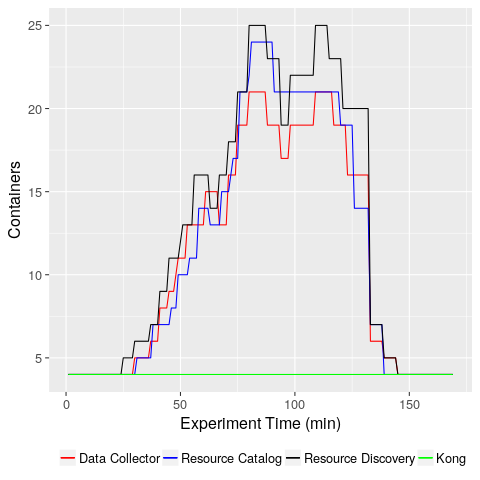
\includegraphics[width=0.7\textwidth]{figuras/auto-scaling.png}
    \caption{Dimensionamento automáticos dos microsserviços da plataforma InterSCity.}
	\label{fig:auto-scaling}
\end{figure}


A Figura \ref{fig:throughput} mostra a taxa de vazão (\textit{throughput}) média da plataforma InterSCity ao longo da duração do experimento.
A taxa de vazão é definida como a taxa de respostas bem sucedidas recebidas pelo componente de integração.
O resultado indica que a taxa de vazão corresponde de perto à carga de trabalho gerada, como pode ser visto comparando as Figuras \ref{fig:workload} e \ref{fig:throughput}.
A plataforma foi capaz de lidar com a demanda variável graças à sua escalabilidade e funcionalidade de dimensionamento automático, descritos na Seção \ref{sec:interscity}.
No entanto, devemos mencionar que a taxa de vazão não correspondeu exatamente à carga de trabalho gerada, pois algumas requisições falharam, representando em média quase 0,6\% de todas as requisições.
As requisições com falha incluem aquelas que tiveram respostas com um código de erro HTTP, bem como aquelas que não foram concluídos devido a recusa de conexão ou \textit{timeout}.
Todavia, consideramos que, ser capaz de lidar com, em média, mais de 99,4\% das requisições sob alta carga é satisfatório; um usuário típico perceberia uma falha a cada 200 requisições, o que é muito bom para
este tipo de aplicação de Cidades Inteligentes em tempo real.

\begin{figure}[ht]
	\centering
	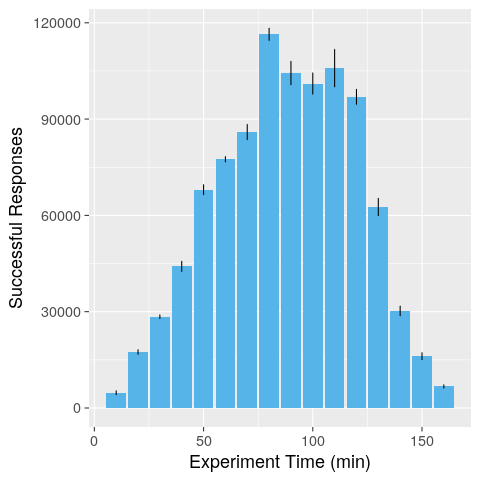
\includegraphics[width=0.7\textwidth]{figuras/throughput.png}
    \caption{Taxa de vazão (\textit{throughput}) média da platafora InterSCity.}
	\label{fig:throughput}
\end{figure}


Outro aspecto fundamental da avaliação de um sistema é analisar o desempenho da plataforma para lidar com requisições de aplicações com uma carga de trabalho variável.
A esse respeito, estamos interessados principalmente em analisar a degradação do desempenho e verificar se a plataforma está sendo dimensionada adequadamente para atender seus clientes dentro de tempos
de resposta aceitáveis.
Para tanto, coletamos o tempo de resposta do ponto de vista do cliente, como mostrado Figura \ref{fig:responsetime}.
Durante a maior parte do experimento, a plataforma foi capaz de responder em menos de um segundo.
No entanto, diferente da taxa de vazão, o impacto do maior período de demanda no tempo de resposta observado é perceptível, uma vez que, durante um intervalo curto (após 110 minutos de execução),
o tempo médio de resposta foi maior que 1 segundo.
O tempo de resposta voltou para 500 milisegundos depois disso.
Entretanto, podemos ver que, mesmo em períodos de alta carga, o tempo de resposta foi mantido abaixo de 2 segundos, o que é um resultado muito bom para esse tipo de aplicação.

\begin{figure}[ht]
	\centering
	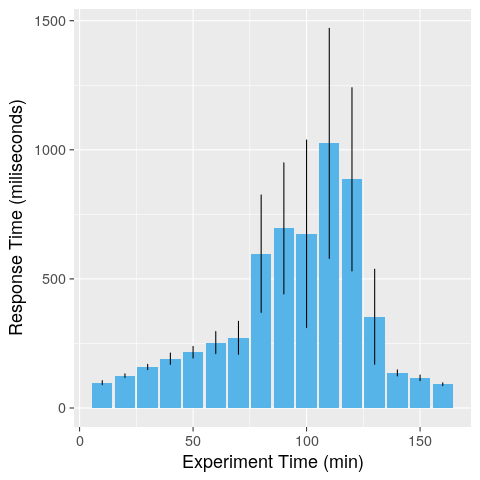
\includegraphics[width=0.7\textwidth]{figuras/response_time_mean.png}
    \caption{Tempo de resposta médio da platafora InterSCity.}
	\label{fig:responsetime}
\end{figure}


Devemos ter em mente que a distribuição de contêineres nos nós disponíveis podem impactar o tempo de resposta, pois vários contêineres podem competir por recursos computacionais se estiverem
sendo executados na mesma máquina.
Além disso, embora o sistema realize a tarefa de dimensionamento automático a cada 30 segundos, não temos controle sobre o tempo que leva para um \textit{container} ser criado, implantado e ficar pronto
para receber novas requisições.
Por outro lado, essa distribuição também pode introduzir um efeito benéfico devido à possível implantação de serviços que constantemente interagem uns com os outros na mesma máquina, reduzindo a latência
de rede e imprevisibilidade.

Ao final desse estudo de caso, percebemos que não exercitamos todos os requisitos apresentados para a construção de um ambiente simulado e integrado para experimentação de plataformas de Cidades Inteligentes.
Por isso, realizamos um segundo estudo de caso, onde a \textbf{atuação} no ambiente simulado se fez necessária, apresentado na seção seguinte.

\section{Tráfego de Carros Inteligente}

Com o objetivo de exercitar o envio de comandos de atuação da plataforma para o ambiente simulado, que não foi explorado no cenário de estacionamento inteligente, definimos um novo cenário.
Neste caso, visamos identificar trechos em vias da cidade com tráfego de carros anômalo (devido ao fechamento de ruas, acidentes, desastres naturais e etc.) e notificar
previamente os motoristas para evitarem passar naquele trecho através de Placas de Mensagens Variadas (PMVs).
Veja na Figura \ref{fig:pmv} uma PMV.
Consideramos aqui uma anomalia uma variação considerável na velocidade média dos carros que trafegam naquele trecho de via naquele horário.
Essas PMVs são posicionadas em pontos estratégicos da cidade e apresentam alertas aos motoristas em tempo real sobre possíveis anomalias no trânsito.
E, com isso, motoristas podem mudar o seu percurso evitando maiores congestionamentos na cidade.

\begin{figure}[ht]
	\centering
	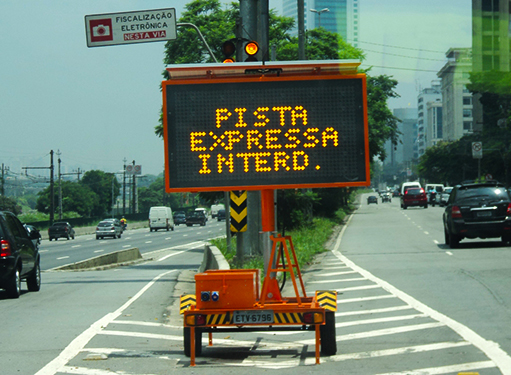
\includegraphics[width=0.7\textwidth]{figuras/pmv.jpg}
    \caption{Exemplo de Placa de Mensagem Variada.}
	\label{fig:pmv}
\end{figure}


A implementação deste cenário seguindo a arquitetura proposta no Capítulo \ref{cap:proposta}, bem como o experimento realizado, serão discutidos nas seções seguintes.

\subsection{Implementação}
\label{sec:smart_traffic}

Essencialmente, o cenário de tráfego de carros inteligente funciona da seguinte forma:

\begin{enumerate}
    \item A plataforma coleta dados históricos de posicionamento dos carros em seus trajetos, a partir desses pontos a velocidade média dos carros é calculada e o método MAD (\textit{Median Absolute Deviation}
        - Desvio Absoluto da Mediana)\citep{leys_2013} é utilizado para definir limiares (\textit{thresholds}) de velocidade média para cada trecho de via da cidade em cada horário, sendo esses limiares
        valores de velocidade média aceitáveis em um dia comum.
        Para isso, o ambiente simulado envia dados de posicionamento georreferenciado dos carros a cada ciclo de execução, simulando por exemplo um dispositivo que contém um
        sistema de GPRS (\textit{General Packet Radio Service}) + GPS (\textit{Global Positioning System}).
        Com uma série de pontos de onde o carro passou em cada instante, se torna possível calcular a sua velocidade média, logo obtemos a velocidade média de carros
        que passaram naquele trecho naquele dado momento durante todo o dia.
        Tendo esses limiares calculados usando o MAD, a plataforma se torna capaz de identificar anomalias na velocidade média dos carros em tempo real, verificando se a variação naquele instante
        extrapola ou não o que foi identificado com os dados históricos.

    \item Ao identifiar uma anomalia de trânsito em algum trecho, a plataforma identifica as PMVs mais próximas do incidente e atualiza a sua mensagem informando os motoristas
        do ocorrido.

    \item Caso o motorista passe por uma PMV contendo essa mensagem, ele verifica se o trecho mencionado faz parte do seu percurso. Sendo verdade, ele recalcula a sua
        rota evitando maiores congestionamentos na região.
\end{enumerate}

Nesse cenário de experimentação, o novo serviço de processamento de dados (históricos e de tempo real), que está em desenvolvimento, e o envio de comandos de atuação da plataforma
InterSCity puderam também ser testados.
Além disso, foi possível finalizar a validação da arquitetura proposta para a criação de um ambiente para experimentação em plataformas de Cidades Inteligentes,
implementando a atuação em tempo real no ambiente simulado.

Para realizar experimentos envolvendo essas funcionalidades da plataforma InterSCity, foi necessário implementar o conceito de PMVs, eventos de fechamentos de via e de
processamento de comandos de atuação em tempo de execuação no InterSCSimulator.
Foi utilizada a publicação de eventos (dados de sensores) implementado para o cenário anterior, já que para o funcionamento do serviço de processamento de dados
em tempo real da plataforma precisamos enviar a cada ciclo de execução da simulação o posicionamento de todos os carros presentes.
Essas funcionalidades são essenciais para atender os \textbf{requisitos fundamentais} para esse cenário.

O modo de publicação de dados em tempo de execução no InterSCSimulator foi refatorado para melhor atender ambos os cenários implementados.
Como visto no cenário anterior, a publicação de eventos da simulação se dava através do agente \textit{Parking Controller} (como pode ser visto na Figura \ref{fig:atualizacao}), já que
até então o único tipo de evento publicado pelo simulador era a atualização da disponibilidade de uma vaga de estacionamento.
No intuito de permitir que outros agentes da simulação também pudessem publicar os seus eventos, um novo agente chamado \textit{Publisher} foi criado, removendo essa responsabilidade
anteriormente atribuída ao agente \textit{Parking Controller}.
%Desse modo, o agente do tipo carro também se tornou capaz de publicar a sua posição, onde a cada ciclo de execução é enviada uma mensagem a um agente \textit{Publisher} contendo sua localização.
Agora, qualquer agente da simulação que deseje publicar um evento deve apenas enviar uma mensagem ao \textit{Publisher} com o conteúdo do evento.
Desse modo, o agente do tipo carro envia a cada ciclo de execução uma mensagem a um agente \textit{Publisher} contendo sua localização, tornando-se capaz de pulicar a sua posição.

Visando tornar factível a simulação de eventos de fechamento de vias na cidade, adicionamos o conceito de eventos de trânsito ao InterSCSimulator.
Um novo arquivo de entrada para o simulador e um novo agente foram adicionados.
O novo arquivo de entrada (chamado por padrão \textit{events.xml}), contem uma lista de eventos de fechamento de via que serão agendados na simulação.
Como pode ser visto na Listagem \ref{code:events}, cada evento é representado por uma lista de atributos separados por ponto e vírgula ('';``), e os atributos são os seguintes:
(i) o tipo do evento de trânsito (\textit{close\_street} para fechamento de vias e \textit{reduce\_capacity} para redução da capacidade de vias);
(ii) o número identificador da via a ser fechada (aresta no grafo da cidade);
(iii) o número do ciclo de simulação onde deve ser iniciado o evento;
(iv) o número de ciclos de simulação que deve durar o evento;
(v) a porcentagem da capacidade do fluxo de carros que ainda estará em funcionamento, usada no caso de um fechamento parcial do trecho (se o evento for de fechamento de via deve-se utilizar o valor 0).
O novo agente chamado \textit{Events Manager} é responsável por agendar todos esses eventos no início da simulação e alterar o grafo da cidade no momento programado.
Quando o trecho da via é fechado, a aresta do grafo da cidade é removida momentaneamnte até o evento ser encerrado, impedindo assim a possibilidade de passagem de qualquer
carro.
Quando o evento apenas reduz a capacidade de fluxo de carros da via, modificamos a sua capacidade para atender o que foi programado até o evento ser encerrado.
Essa capacidade é um atributo dado àquela aresta do grafo.

\lstset{
    language=xml,
    tabsize=3,
    frame=lines,
    caption=Arquivo de entrada contendo os eventos de fechamento de vias,
    label=code:events,
    frame=shadowbox,
    rulesepcolor=\color{gray},
    xleftmargin=20pt,
    framexleftmargin=15pt,
    keywordstyle=\color{blue}\bf,
    commentstyle=\color{OliveGreen},
    stringstyle=\color{red},
    numbers=left,
    numberstyle=\tiny,
    numbersep=5pt,
    breaklines=true,
    showstringspaces=false,
    basicstyle=\footnotesize,
    emph={uuid,node},emphstyle={\color{magenta}}}
    \lstinputlisting{files/events.csv}

Para a representação das PMVs no InterSCSimulator, foi criado um agente chamado \textit{PMV Manager}.
Seu papel é atualizar as mensagens de PMVs.
As PMVs em si foram implementadas como atributos de vértices do grafo da cidade (sendo os vértices o encontro de duas ou mais vias).
Nesse atributo, é guardada uma lista de trechos de vias (arestas) onde foram encontradas alguma anomalia no trânsito.
Os agentes do tipo carro, ao passar por um vértice que contém esse atributo, verificam se alguma das arestas ali presentes fazem parte do seu trajeto ou não.
Caso positivo, o seu percurso é recalculado.
Caso contrário, ele se mantém inalterado.

A última implementação no InterSCSimulator necessária para atender os requisitos apresentados seguindo a arquitetura proposta foi o recebimento de comandos de atuação e
seu processamento em tempo de execução.
Essa funcionalidade é fundamental para a atualização das PMVs em tempo de execução pela plataforma.
Diante disso, mais um novo agente foi criado para ficar à espera desses comandos enviados pela plataforma: o \textit{Listener}.
Como um comando de atuação pode ser enviado a qualquer momento, foi necessário criar esse novo agente, cuja única responsabilidade é receber esse comando e armazená-lo em uma
estrutura de dados, para que outros agentes não ficassem bloqueados (bloqueando também a simulação) a espera de tal acontecimento.
Ou seja, esse agente fica em um laço (\textit{loop}) infinito a espera de uma mensagem que é enviada via AMQP (mesmo protocolo utilizado para publicação dos dados).
%A utilização do RabbitMQ foi escolhida devido a possibilidade da plataforma InterSCity enviar comandos de atuação através do mesmo, e como foi uma funcionalidade nova,
%decidimos utilizar a mesma tecnologia, reduzindo assim o problema de interoperabilidade.
Por essa ser uma nova funcionalidade, decidimos utilizar o mesmo protocolo e a mesma tecnologia utilizada pela plataforma InterSCity visando reduzir o problema de interoperabilidade.
O RabbitMQ, que já vinha sendo utilizado pela plataforma para envio de comandos de atuação, foi selecionado como ferramenta para tratamento de eventos da simulação, tanto para publicação quanto para 
recebimento.
Quando um comando é recebido, no caso uma aresta de trecho anômalo a ser atualizada em uma PMV, o \textit{Listener} armazena essa mensagem em uma estrutura de dados que é acessada no
próximo ciclo de execução pelo \textit{PMV Manager} que, por sua vez, atualiza o atributo da referida PMV (vértice no grafo).

Após a apresentação das funcionalidades e melhorias implementadas, as duas vias de fluxo de comunicação entre o simulador e a plataforma serão apresentadas a seguir.
Na Figura \ref{fig:smart_traffic_publish_data}, os passos para a publicação dos dados de posicionamento de cada um dos carros a cada ciclo de execução são expostos.

\begin{figure}[ht]
	\centering
	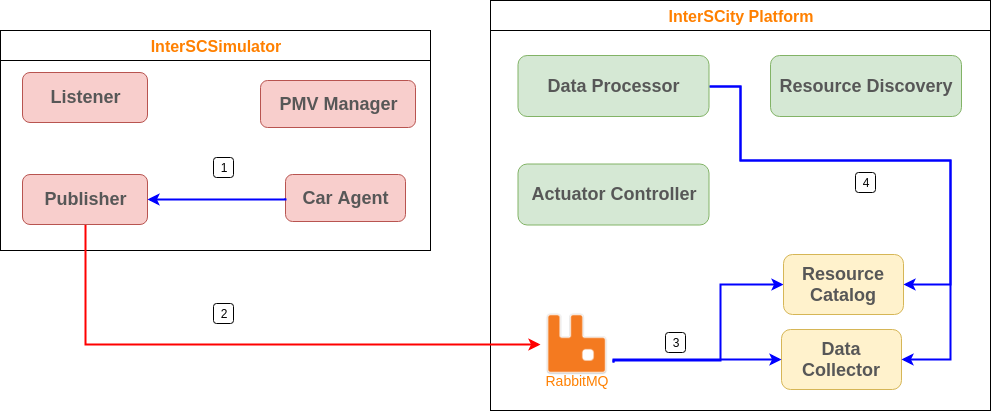
\includegraphics[width=\textwidth]{figuras/integration-publish-car-position.png}
	\caption{Integração para publicar dados de posicionameto de carros}
	\label{fig:smart_traffic_publish_data}
\end{figure}

\begin{enumerate}
    \item O agente do tipo carro a cada ciclo de execução envia uma mensagem para o agente \textit{Publisher} contendo a sua posição naquele dado momento.

    \item O agente \textit{Publisher} se conecta ao \textit{broker} do RabbitMQ e publica uma mensagem contendo: o identificador do carro, o seu posicionamento e o \textit{timestamp}.

    \item Os microsserviços \textit{Resource Catalog} e \textit{Data Collector} são notificados e recebem tais dados. O \textit{Resource Catalog} atualiza o último dado monitorado
        daquele carro, e o \textit{Data Collector} atualiza a sua base de dados contendo todas as medições.

    \item O microsserviço \textit{Data Processor} acessa dados armazenados por esses outros serviços com o intuito de definir limiares para velocidade média de vias (dados históricos),
        ou para identificar anomalias no trânsito (fluxo de dados em tempo real).
\end{enumerate}

Já na Figura \ref{fig:smart_traffic_actuation}, é apresentado o fluxo para atualização da lista de trechos anômalos de vias em PMVs, representando aqui um comando de atuação no
ambiente simulado.
Lembrando que o gatilho para a execução desse processo é o serviço de processamento de dados identificar alguma anomalia no trânsito.

\begin{figure}[ht]
	\centering
	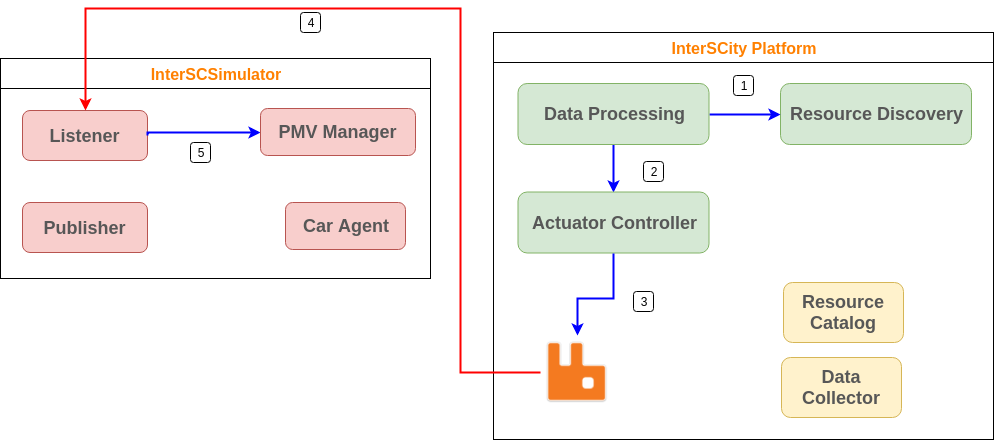
\includegraphics[width=\textwidth]{figuras/integration-actuate-pmv.png}
	\caption{Integração para atuação em Placas de Mensagens Variadas}
	\label{fig:smart_traffic_actuation}
\end{figure}

\begin{enumerate}
    \item O \textit{Data Processor}, ao identificar uma anomalia no trânsito em determinado ponto da cidade, requisita ao \textit{Resource Discovery} as PMVs mais próximas
        daquele ponto, para que elas possam ser atualizadas.

    \item Ao serem identificados as PMVs, o \textit{Data Processor} envia os identificadores das PMVs e do trecho anômalo para o \textit{Actuator Controller}.

    \item O \textit{Actuator Controller} formata essas mensagens e as publica em um dos canais do RabbitMQ.

    \item O agente \textit{Listener}, cujo único papel é esperar por esse tipo de mensagem, a recebe e a armazena em uma estrutura de dados compartilhada pelos agentes do simulador.

    \item O agente \textit{PMV Manager} verifica a presença dessa nova mensagem na estrutura de dados compatilhada, e atualiza o atributo que representa a PMV no vértice do grafo
        viário da cidade, adicionando mais esse trecho para a lista presente ou criando-a caso não exista nenhum outro trecho.
\end{enumerate}

Um ponto interessante desse segundo cenário, foi a não necessidade de um componente de integração, já que ambas as ferramentas se comunicam através do mesmo protocolo (inclusive a
mesma ferramenta) e conseguem representar os mesmos conceitos de maneira equivalente.
Esse é o cenário ideal para criação de um ambiente simulado de experimentação para uma plataforma de Cidades Inteligentes, já que não foi essencial a implementação desse
componente extra que, como discutido, traria mais complexidade para o sistema, podendo aumentar o tempo de resposta entra as ferramentas.
Claro que tudo isso foi possível porque neste mesmo trabalho fizemos toda a implementação dos \textbf{requisitos fundamentais} apresentados, portanto,
tivemos a oportunidade de tomar as decisões técnicas que facilitaram a integração entre as duas ferramentas.


\subsection{Experimento}

Esse experimento consistiu em três cenários.
Conforme descrito na Seção \ref{sec:smart_traffic}, limiares (\textit{thresholds}) de velocidade média para cada trecho de via em cada horário do dia deveriam ser definidos.
Portanto, o primeiro cenário consistiu na simulação do trânsito da cidade sem nenhum evento de fechamento de via, ou seja, o trânsito normal da cidade.
Para tanto, a aplicação de detecção de anomalias foi capaz de, com os dados de posicionamento de carros enviados a cada ciclo de execução, definir esses tais limiares através do método MAD.
O segundo cenário, consistiu em simular o trânsito de carros na cidade com alguns eventos de fechamento de vias (representando ruas alagadas, acidentes de carro, etc.).
Nesse cenário, simulamos o comportamento caótico visto nas grandes cidades, onde vias são interditadas e interferem diretamente no tráfego dos carros.
No último cenário, simulamos o mesmo comportamento do segundo cenário, mas adicionamos as PMVs para auxiliar os condutores de carros a contornar tais situações.
Tendo em vista que os limiares já haviam sido definidos, a aplicação, sem ter conhecimento prévio dessas vias fechadas, detectava automaticamente esses trechos e notificava os motoristas através da
atualização de mensagens nas PMVs.
O objetivo desses três cenários era verificar o impacto do uso de PMVs no tempo de duração médio das viagens de carro em situações de incidentes que inviabilizam a utilização de certas vias em uma cidade.

Para verificar o bom funcionamento desse cenário no ambiente simulado, dividimos esse experimento em dois.
Na primeira parte, realizamos um experimento numa escala menor e com dados fictícios, visando meramente a validação do comportamento esperado e interação entre os componentes.
Na segunda parte, utilizamos dados abertos da cidade de São Paulo, aumentando a escala do experimento e se aproximando de um cenário mais realista.
O código fonte para a execução do experimento e a análise apresentada, nesta seção, estão disponíveis em nosso repositório aberto
\footnote{https://github.com/LSS-USP/pmv\_experiment/blob/master/Analysis.ipynb}.

\subsubsection{Validação}

Nesse experimento inicial de validação, os três cenários com o que diz respeito ao número de eventos de fechamento de via e PMVs, se deram da seguinte forma:

\begin{enumerate}
    \item Sem eventos de fechamento de via e sem PMVs

    \item Com um evento de fechamento de via e sem PMVs

    \item Com um evento de fechamento de via e uma PMV
\end{enumerate}

Foram executadas 20 iterações de cada uma dos cenários, onde em cada iteração corresponde a 10 minutos de simulação.
Em todos os cenários, utilizamos um grafo com 8 vértices e 16 arestas, como pode ser visto na Figura \ref{fig:mapa_validacao}.
O grafo é direcionado, onde cada aresta na verdade representa duas, sendo uma entrando e outra saíndo de seus vértices, ou seja, simbolizam vias de mão dupla.

\begin{figure}[ht]
	\centering
	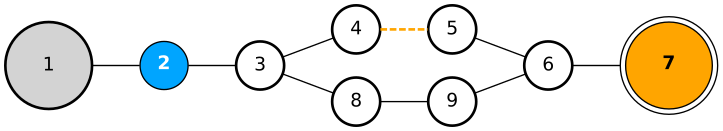
\includegraphics[width=\textwidth]{figuras/mapa_validacao.png}
	\caption{Mapa viário da cidade utilizado para validação.}
	\label{fig:mapa_validacao}
\end{figure}

O grafo da Figura \ref{fig:mapa_validacao} retrata o mapa viário da cidade simulada da seguinte forma:

\begin{itemize}
    \item Os vértices representam início e/ou fim de uma ou mais ruas.

    \item As arestas representam segmentos de vias da cidade.

    \item Todas as arestas possuem comprimento 1. Por isso, a cada ciclo de simulação, caso seja possível, um carro percorre uma aresta.
\end{itemize}

Além disso, adotamos a seguinte forma para separar vértices e arestas que desempenham papel importante neste experimento:

\begin{itemize}
    \item A aresta pontilhada amarela representa a via da cidade que será fechada durante a simulação (essa aresta só será afetada nos cenários que posssuem tal evento).

    \item O vértice 1 (em cinza) representa a origem de todas as viagens simuladas.

    \item O vértice 7 (em alaranjado) representa o destino das viagens.

    \item O vértice 2 (em azul) representa o local da cidade que contém uma PMV que alertará os motoristas sobre possíveis anomalias nas vias.
\end{itemize}

Em todas as iterações de todos os cenários, simulamos um total de 100 carros realizando viagens partindo do vértice 1 até o 7, onde metade dos carros partem no início da simulação e o restante após 50 ciclos
de execução.
Como o intuito desse experimento era validar o comportamento da implementação do ambiente de experimentação como um todo, antes de apresentar os resultados obtidos, descrevemos o resultado esperado para
cada um dos cenários a seguir.

Na Figura \ref{fig:mapa_etapa1}, pode-se ver o caminho esperado que os carros percorrecem no primeiro cenário do experimento, onde não há a presença de eventos de fechamento de vias, e muito menos PMV.
As arestas em \textbf{roxo} representam o trajeto do carro, as demais arestas não utilizadas foram removidas do grafo a título de legibilidade.
Note que ao chegar no vértice 3, ele sempre optará o caminho seguindo pelo vértice 4.
Isso acontece porque todas as arestas possuem o mesmo comprimento (ambos são um caminho mais curto até o destino), sendo critério de desempate o menor índice.

\begin{figure}[ht]
	\centering
	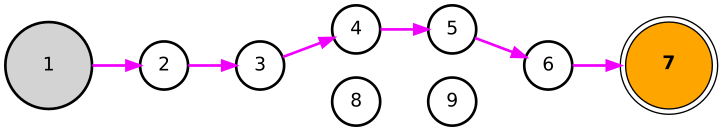
\includegraphics[width=\textwidth]{figuras/mapa_etapa1.png}
	\caption{Trajeto esperado do cenário 1 do experimento.}
	\label{fig:mapa_etapa1}
\end{figure}

Na Figura \ref{fig:mapa_etapa2}, o trajeto esperado para que o carro percorra no cenário 2 do experimento é apresentado.
Nesse cenário, temos uma via fechada, sendo ela entre os vétices 4 e 5, e nenhuma PMV para auxiliar os motoristas.
Em \textbf{roxo} podemos ver as arestas que serão percorridas inicialmente;
em cor \textbf{preta}, as arestas que faziam parte do caminho inicialmente calculado, mas que não foram percorridas devido ao fechamento da via (aresta tracejada);
e em cor \textbf{verde}, o caminho recalculado após se deparar com o fechamento de via no vértice 4.

\begin{figure}[ht]
	\centering
	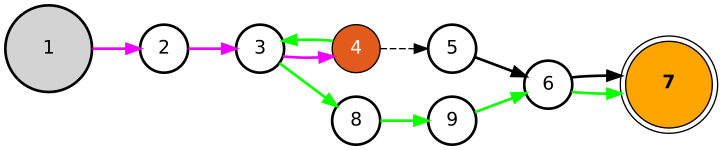
\includegraphics[width=\textwidth]{figuras/mapa_etapa2.png}
	\caption{Trajeto esperado do cenário 2 do experimento.}
	\label{fig:mapa_etapa2}
\end{figure}

Por fim, na Figura \ref{fig:mapa_etapa3}, temos a dinâmica esperada para o cenário 3, onde existe o fechamento da via. Contudo, a PMV se faz presente para notificar os condutores de veículos.
Mais uma vez, a via representada pela aresta 4 -> 5 é fechada, e a PMV é posicionada no vértice 2 representado em azul.
Utilizamos aqui a mesma notação anterior.
A aresta \textbf{roxa} representa o caminho inicialmente calculado e que foi percorrido;
as arestas \textbf{pretas} faziam parte do caminho inicial, mas nesse caso não foram percorridas devido ao fechamento da via e da PMV;
e as \textbf{verdes} simbolizam o novo caminho recalculado após o motorista ter sido notificado pela PMV.
No modelo implementado, ainda assim, era esperado que alguns carros percorresem o fluxo apresentado na Figura \ref{fig:mapa_etapa2}, já que acreditamos que nem todos os motoristas que vissem
a notificação iriam de fato mudar o seu trajeto.

\begin{figure}[ht]
	\centering
	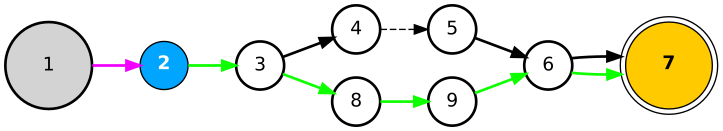
\includegraphics[width=\textwidth]{figuras/mapa_etapa3.png}
	\caption{Trajeto esperado do cenário 3 do experimento.}
	\label{fig:mapa_etapa3}
\end{figure}

Os três cenários desse experimento foram realizados em dois \textit{laptops} com 8 CPUs virtuais (1.80 GHz) e 8 GB de memória RAM.
Diferente do experimento apresentado na Seção \ref{sec:exp_smart_parking}, o foco desse experimento não é analisar o desempenho da plataforma, mas sim uma análise funcional. 
Os passos para execução desse experimento de validação foram os seguintes:

\begin{enumerate}
    \item Executar uma instância em modo de produção da plataforma InterSCity em um \textit{laptop}.

    \item Executar uma instância em modo de produção do simulador InterSCSimulator no outro \textit{laptop}.

    \item Configurar rede local entre os \textit{laptops}, conectados de maneira cabeada via ethernet.

    \item Realizar a simulação do cenário de tráfego inteligente de carros.

    \item Analizar os resultados obtidos ao final da simulação.
\end{enumerate}

A Figura \ref{fig:distancia_validacao}, apresenta a distância média percorrida pelos carros simulados nos três cenários deste experimento.
De acordo com as nossas hipóteses, esperávamos que os carros no cenário sem evento de fechamento de via e sem PMV para notificar os motoristas, percorressem 6 arestas, no cenário com evento e sem PMV
percorressem 8 arestas e no cenário com evento e PMV percorressem entre 6 e 8 arestas (alguns veículos ignoram as notificações).
Nossas hipóteses foram confirmadas, conforme o gráfico.

\begin{figure}[ht]
	\centering
	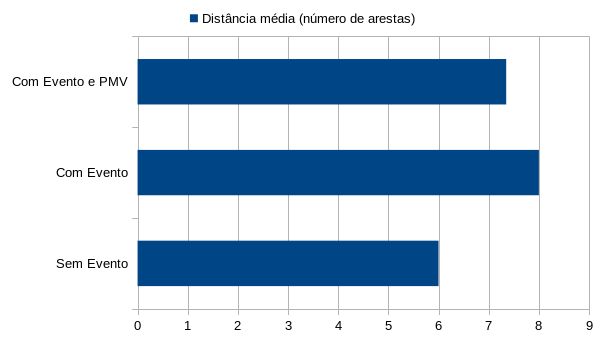
\includegraphics[width=\textwidth]{figuras/distancia_validacao.png}
	\caption{Média da distância percorrida pelos carros no experimento.}
	\label{fig:distancia_validacao}
\end{figure}

Uma análise semelhante foi realizada com a duração das viagens simuladas, como pode ser visto na Figura \ref{fig:duracao_validacao}.
As durações média das viagens simuladas nos três cenários do experimento são apresentadas no gráfico.
Uma viagem dura sempre 2 ciclos de execução (criação e destruição do ator) mais o tempo utilizado para percorrer as arestas (uma aresta por ciclo de execução, já que possuem comprimento unitário)
e o recálculo de um caminho dura um ciclo.
Por isso, esperávamos que para o cenário sem evento de fechamento de via durasse 8 ciclos (2 pelo ciclo de vida + 6 arestas);
o cenário com evento e sem PMV, para informar os motoristas, durasse 11 ciclos (2 pelo ciclo de vida + 8 arestas + 1 pelo recálculo da rota);
e o cenário com evento e PMV durasse entre 9 ciclos (2 pelo ciclo de vida + 6 arestas + 1 pelo recálculo) para motoristas que seguissem as instruções da PMV, e 11 ciclos (2 pelo ciclo de vida + 8 arestas +
1 pelo recálculo) para os motoristas que ignorassem a PMV.
Nossas hipóteses mais uma vez foram confirmadas, como pode ser visto na Figura \ref{fig:duracao_validacao}.

\begin{figure}[ht]
	\centering
	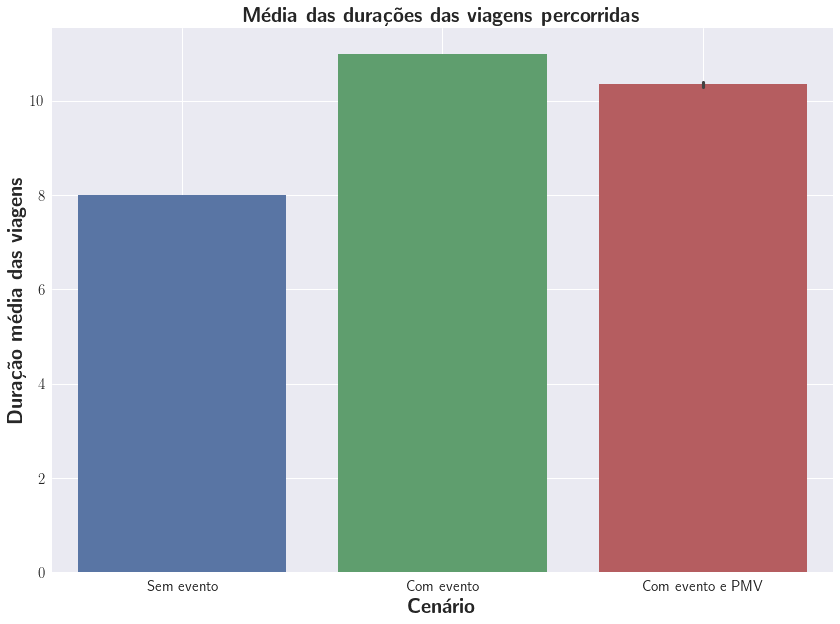
\includegraphics[width=\textwidth]{figuras/duracao_validacao.png}
	\caption{Média da duração das viagens simuladas no experimento.}
	\label{fig:duracao_validacao}
\end{figure}

Com isso, pudemos verificar os requisitos fundamentais e de integração, apresentados na Seção \ref{sec:requisitos}, para este cenário de tráfego de carros inteligentes.
O modelo implementado no simulador correspondeu com o esperado e a comunicação entre as ferramentas foi validada, principalmente com o que diz respeito à atuação no ambiente simulado, sendo esse um
trabalho pioneiro.

\subsubsection{Cidade de São Paulo}
\label{sec:smart_traffic}

Tendo em vista que a implementação dos modelos utilizados para este cenário e a integração estavam funcionando dentro do esperado, realizamos um outro experimento, envolvendo o mesmo cenário de tráfego 
inteligente de carros, mas dessa vez em uma escala maior, com dados abertos da cidade de São Paulo.

Dividimos esse experimento em três cenários novamente, quanto ao número de eventos de fechamento de via e PMVs. Eles se deram da seguinte forma:

\begin{enumerate}
    \item Sem eventos de fechamento de via e sem PMVs

    \item Com eventos de fechamento de via e sem PMVs

    \item Com eventos de fechamento de via e 7 PMVs
\end{enumerate}

Foram executadas 20 iterações de cada uma dos cenários e, em cada iteração, simulamos 1 hora e 30 minutos.
Neste experimento, utilizamos dados do OpenStreet Maps e a pesquisa Origem-Destino realizado pela companhia de metrô da cidade de São Paulo em 2007 para definição do cenário a ser simulado.
A seguir mais detalhes sobre esses dados.

Dessa vez, não utilizamos o mapa viário completo da cidade de São Paulo.
Realizamos um recorte de um trecho da avenida Rebouças com um raio de 5km, próximo ao cruzamento da avenida Paulista.
O intuito desse recorte era reduzir o escopo do experimento para enfatizar o impacto das PMVs naquela região.
Para a criação das viagens de carros a serem realizadas, utilizamos os mesmos dados da pesquisa OD (Origem-Destino) apresentada no experimento de estacionamento inteligente.
Contudo, como não utilizamos o mapa completo da cidade, filtramos apenas as viagens em que a origem e o destino pertencessem ao recorte do mapa realizado.
Todos os \textit{scripts} utilizados para filtrar os dados de entrada estão disponíveis em nosso repositório aberto\footnote{https://github.com/LSS-USP/pmv\_experiment}.

\begin{itemize}
    \item \textbf{OpenStreet Maps}: para criar o grafo viário da cidade de São Paulo usado na simulação, utilizamos o mapa do OpenStreet Maps.
        Este mapa contém todas as ruas e junções da cidade, em conjunto com um vasto número de atributos, como comprimento, capacidade e velocidade limite.
        Tais informações são usadas pelo simulador para definir as rotas percorridas pelos carros durante a realização de suas viagens, bem como simular o impacto do tráfego na velocidade dos carros.

    \item \textbf{Pesquisa Origem-Destino (OD)}: criamos as viagens de carro simuladas com base na pesquisa OD realizada pela Companhia de Metrô de São Paulo.
        \footnote{Pesquisa Origem-Destino - http://goo.gl/Te2SX7.}
        Essa pesquisa descreve as viagens de 200.000 pessoas e extrapola os dados para toda a população da cidade.
        A pesquisa inclui informações sobre a origem, o destino, o modo de transporte e a hora de partida.
        Esses dados foram empregados para definir o comportamento dos agentes do tipo carro na simulação.
        Simulamos o tráfego em São Paulo durante o horário das 8h às 9h30.
        Na pesquisa OD, há 2.210 viagens de carro que começam durante o intervalo de tempo considerado e no recorte do mapa feito.
\end{itemize}

No cenário 3 deste experimento, onde fizemos uso de 7 PMVs, posicionamos os mesmos nas principais vias presentes no recorte do mapa, como pode ser visto na Figura \ref{fig:pos_pmvs}.
Decidimos sinalizar tais vias acreditando que por possuírem um maior fluxo de carros, possivelmente impactariam nas rotas de mais carros.

\begin{figure}[ht]
	\centering
	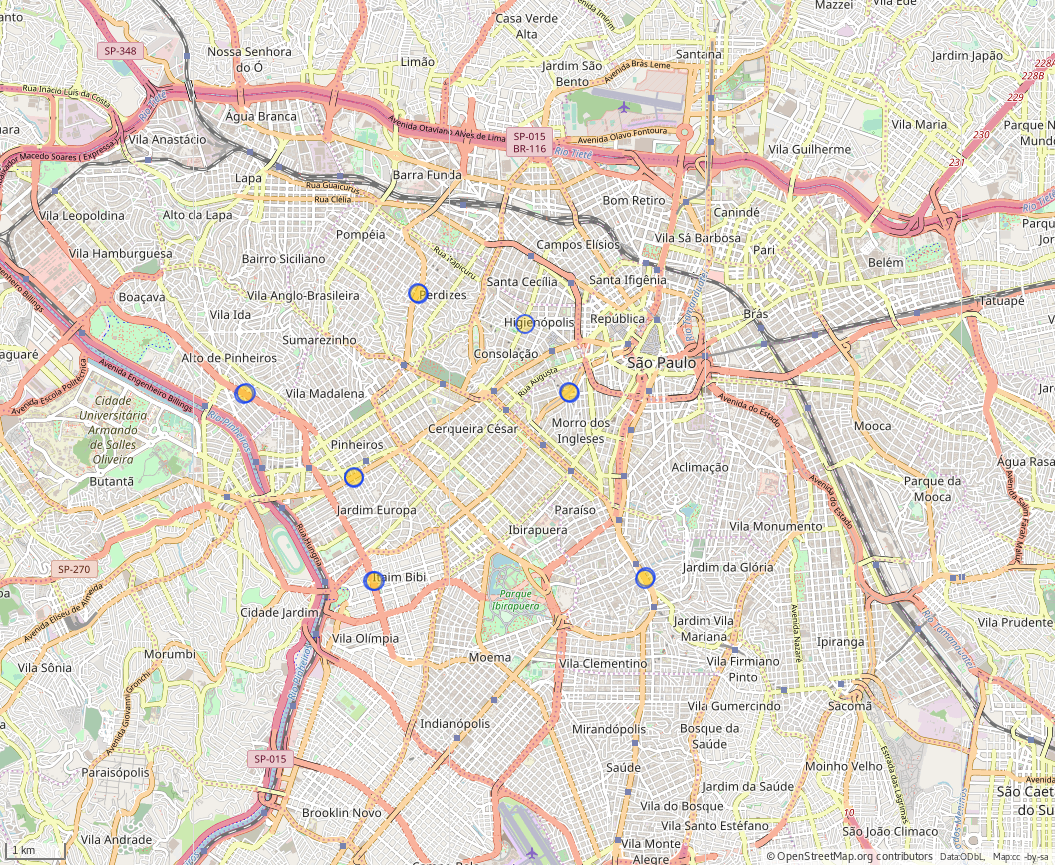
\includegraphics[width=.7\textwidth]{figuras/pmvs_locations.png}
	\caption{Posicionamento das PMVs no experimento de tráfego inteligente de carros.}
	\label{fig:pos_pmvs}
\end{figure}

Na Figura \ref{fig:eventos}, pode-se ver os trechos de vias que foram fechadas nos cenários 2 e 3 deste experimento.
No grafo do mapa viário da cidade gerado a partir do OpenStreet Maps, uma mesma via é formada de várias pequenas arestas (segmentos de via).
Visando enfatizar um evento como um acidente de carro fatal ou um possível alagamento na região, fechamos um conjunto de arestas nas proximidades das avenidas Rebouças e Paulista.

\begin{figure}[ht]
	\centering
	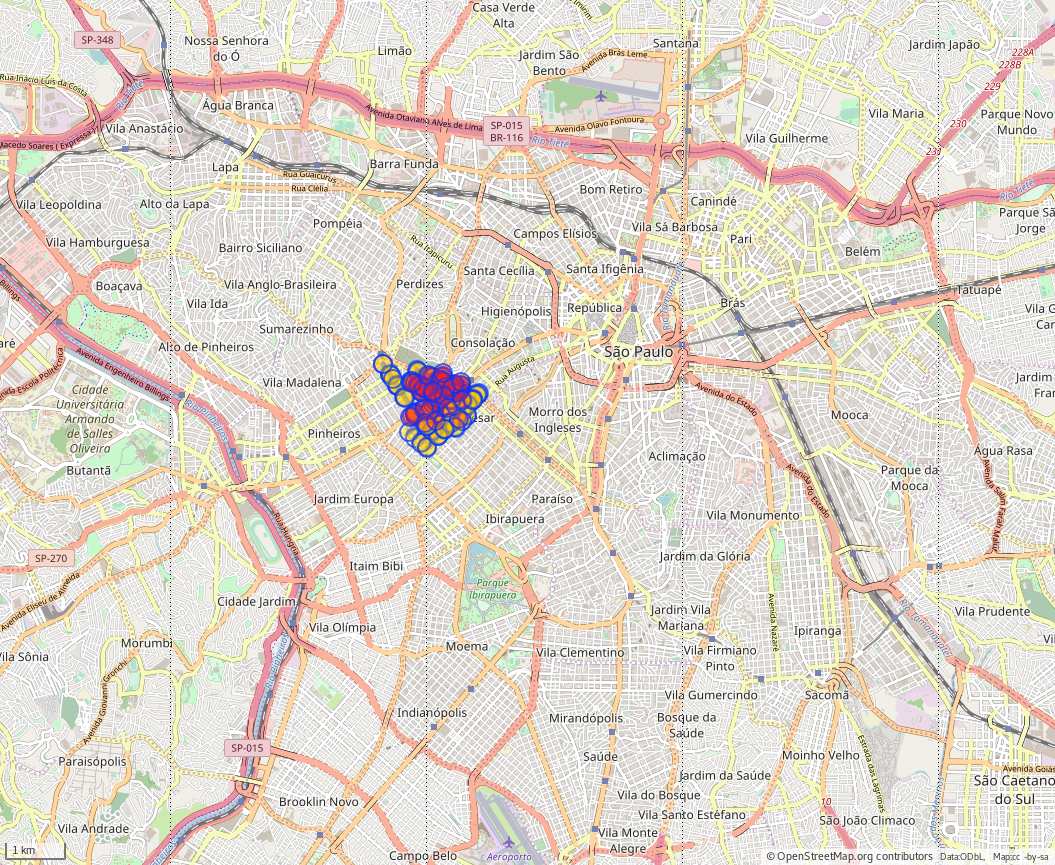
\includegraphics[width=.7\textwidth]{figuras/events_edges_map.png}
	\caption{Local dos eventos de fechamento de via no experimento de tráfego de carros inteligente.}
	\label{fig:eventos}
\end{figure}

Sabendo o local dos eventos de fechamento de vias e o posicionamento das PMVs, esperávamos que a notificação prévia dos motoristas sobre o acidente reduzisse a média do tempo de viagem dos motoristas
com relação a não existência das PMVs.
Consideramos que, pelo fato das avenidas Rebouças e Paulista serem bem movimentadas, muitas das viagens simuladas neste experimento passassem por aquele trecho. 
Contudo, a utilização das PMVs não deveria melhorar a média da duração das viagens em relação ao cenário onde não acontece nenhum evento de fechamento de via.

Os três cenários desse experimento foram realizadas novamente em dois \textit{laptops} com 8 CPUs virtuais (1.80 GHz) e 8 GB de memória RAM.
Mais uma vez, diferente do experimento apresentado na Seção \ref{sec:exp_smart_parking}, o foco desse experimento não é analisar o desempenho da plataforma, mas sim uma análise funcional. 
Os passos para execução desse experimento foram os seguintes:

\begin{enumerate}
    \item Executar uma instância em modo de produção da plataforma InterSCity em um \textit{laptop}.

    \item Executar uma instância em modo de produção da simulador InterSCSimulator no outro \textit{laptop}.

    \item Configurar rede local entre os \textit{laptops}, conectados de maneira cabeada via ethernet.

    \item Realizar a simulação do cenário de tráfego de carros inteligente.

    \item Analizar os resultados obtidos ao final da simulação.
\end{enumerate}

A Figura \ref{fig:duracao_total}, apresenta a duração média das viagens de carro simuladas nos três cenários deste experimento.
No eixo X, a duração é apresentada em segundos (ciclo de execução da simulação: 1 ciclo = 1 segundo), e no eixo Y os três cenários do experimento.
Como podemos ver no gráfico apresentado, em geral, a média do tempo de duração das viagens não passou de 6 minutos.
Isso pode ter ocorrido pelo fato das viagens nessa região serem mais curtas, ou por não terem viagens suficientes para gerar congestionamentos, já que filtramos apenas as viagens que se iniciavam e
terminavam dentro do recorte do mapa utilizado.
Outro fator importante que nos chamou a atenção, foi a média da duração das viagens do cenários 3 (onde existem vias fechadas e o auxilio de PMVs) ser menor do que do cenário 1 (onde não existe qualquer
incidente).
Após analisar os dados, percebemos que ao recalcular a rota, na presença de uma PMV, os carros se distribuíam de uma melhor forma pela malha viária do cenário utilizado pelo experimento, com isso,
evitavam congestionamentos que ocorriam anteriormente.
Sendo isso um alvo de possível melhoria no simulador, já que ao criar o ator, apenas um dos menores caminhos entre a origem e destino do carro é calculado e utilizado, podendo essa rota coincidir entre
múltiplos atores com origem e destinos similares, assim, deixando outros caminhos mais curtos inutilizados.
Todavia, como esperado, o cenário 2, onde temos fechamento de vias mas não temos PMVs, teve a maior média de duração das viagens.

\begin{figure}[ht]
	\centering
	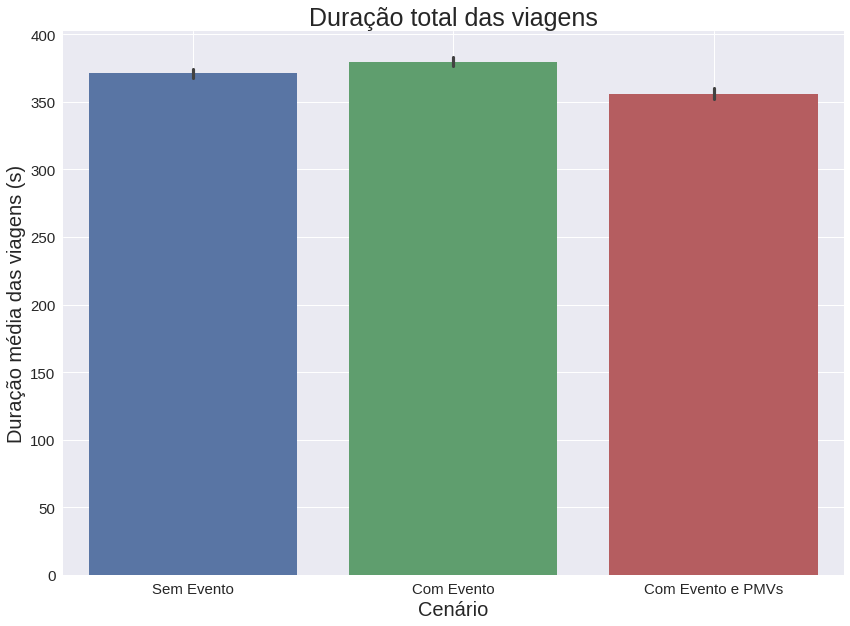
\includegraphics[width=\textwidth]{figuras/duracao_total.png}
	\caption{Média da duração das viagens de carros no experimento.}
	\label{fig:duracao_total}
\end{figure}

Para garantirmos uma melhor acurácia na análise dos resultados obtidos, filtramos apenas as viagens que foram influencidas de alguma forma pelo fechamento de vias e/ou PMVs.
Isso porque percebemos a existência de viagens que não eram modificadas em nenhum dos cenários do experimento, ou seja, a sua duração era sempre a mesma.
Na Figura \ref{fig:duracao_filtered}, apresentamos o mesmo gráfico discutido anteriormente, só que incluindo apenas as viagens que foram afetadas.
Agora analisando o gráfico com as viagens afetadas, obtivemos o resultado esperado no início do experimento.
O cenário 1, onde não há vias fechadas, teve o menor tempo médio de duração de viagens, sendo esse o nosso limite inferior.
O cenário 2, onde vias foram fechadas, o pior tempo médio de viagem foi obtido, sendo o limite superior.
E o cenário 3, onde introduzimos as PMVs para auxiliar os motoristas na decisão da melhor rota a seguir, apresentou um tempo médio de viagem ligeiramente menor do que o cenário 2 e maior do que o cenário 1.

\begin{figure}[ht]
	\centering
	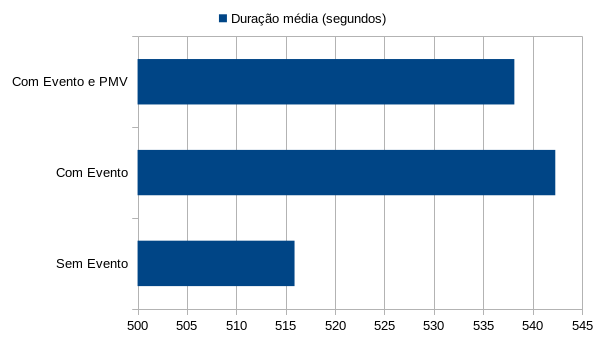
\includegraphics[width=\textwidth]{figuras/duracao_filtered.png}
	\caption{Média da duração das viagens de carros afetadas por fechamento de vias e/ou PMVs no experimento.}
	\label{fig:duracao_filtered}
\end{figure}

Contudo, a melhora de aproximadamente 5\% na média do tempo de duração da viagem do cenário 3 com relação ao cenário 2 não foi um resultado expressivo.
Avaliamos que alguns fatores podem ter influenciado nesse resultado, sendo a maioria deles voltado para os dados utilizados para a definicação do cenário de simulação deste experimento.
O posicionamento das PMVs pode não ter sido o ideal, já que não foi realizada uma análise prévia de onde passariam a maior parte dos carros.
O conjunto de viagens simulados após recortar o mapa da cidade de São Paulo pode não ter sido representativo, a decisão de reduzir o mapa para facilitar a visualização do impacto do fechamento de vias
e PMVs pode não ter sido boa ideia.
Além disso, os resultados obtidos podem ter sido influenciados devido à infraestrutura simples utilizada com apenas dois \textit{laptops}, já que em cenários realistas muitos recursos computationais são
necessários, como memória e largura de banda da rede.


\section{Discussão}

% Melhorias, o que fucionou, o que não funcionou

Após a realização dos dois estudos de caso apresentados neste capítulo, foi possível perceber que a solução proposta no Capítulo \ref{cap:proposta} é viável e nos permitiu realizar
diferentes experimentos utilizando um ambiente simulado de uma cidade, podendo substituir \textit{testbeds} reais e aumentando a escala dos experimentos.
Contudo, durante a implementação dos dois cenários de Cidades Inteligentes apresentados, algumas adversidades foram encontradas e solucionadas.
A fim de contribuir com trabalhos futuros que sigam a solução proposta, uma discussão sobre os principais problemas e dificuldades encontradas será feita
nesta seção.
O intuito aqui é enfatizar os principais obstáculos a serem enfrentados durante a implementação de novos cenários no ambiente integrado usando o simulador InterSCSimulator e
a plataforma InterSCity ou até mesmo envolvendo outras ferramentas, bem como discutir os resultados experimentais alcançados nos estudos de caso.


\subsection{Implementação da Solução Proposta}

Como vem sendo discutido no decorrer deste trabalho, a integração de ferramentas não é algo trivial.
Apesar de tanto o simulador quanto a plataforma utilizada serem voltados para o contexto de Cidades Inteligentes, na maioria das vezes, elas não são concebidas inicialmente
para serem integradas com outras ferramentas.
Através dos próprios requisitos apresentados podemos antever o maior desafio a ser enfrentado: a interoperabilidade.
Essa tanto a nível de comunicação quanto semanticamente.

Como constatado na implementação dos dois cenários apresentados, tentamos ao máximo reduzir a responsabilidade do componente de integração, que ao ser atribuído muitas
tarefas pode se tornar um problema.
Tanto que não foi necessária a implementação desse componente no segundo estudo de caso, tendo em vista que as ferramentas já atendiam os requisitos de integração.
Isso pode ser atribuído ao fato de ambas as ferramentas (InteSCSimulator e InterSCity) serem mantidas pelo nosso grupo de pesquisa, onde tivemos a liberdade de evoluir o
que foi preciso nas próprias ferramentas para facilitar a integração.
Em um contexto onde não existisse essa flexibilidade, o desafio se tornaria bem mais complexo.

Mesmo assim, enfrentamos problemas principalmente com a escalabilidade da solução.
Em experimentos anteriores e isolados, foi demonstrado que ambas as ferramentas eram escaláveis, se comportando bem diante de uma grande carga de trabalho.
Entretanto, a integração traz alguns elementos extras que, por menor que sejam, interferem em cenários de larga escala.
Em experimentos na escala de uma cidade como São Paulo, qualquer mínimo detalhe é potencializado.
Semanticamente não tivemos muitos problemas, já que ambas as ferramentas foram implementadas seguindo conceitos similares, devido a própria sinergia do grupo de
pesquisa.
Todavia, a comunicação entre as ferramentas foi a raíz da maior parte dos problemas enfrentados.

Inicialmente, tentamos realizar qualquer interação com a plataforma através de requisições HTTP, usando a sua API \textit{Restful}.
Contudo, percebemos que o componente de integração necessitaria de uma complexidade muito maior para tratar todas essas requisições paralelamente sem se tornar um
gargalo para o sistema.
Por isso, decidimos explorar bastante o protocolo AMQP através da implementação do RabbitMQ.
Essa se apresentou uma solução mais simples, já que o \textit{broker} do RabbitMQ trata todas essas questões de escalabilidade de maneira eficiente, sendo essa
uma solução adotada pelo mercado.
Além do mais, pelo fato da comunicação via AMQP ser assíncrona e pela própria natureza dos cenários implementados, diferente de requisições HTTP, ela se apresentou uma
solução mais adequada, não bloqueando agentes da simulação a espera de respostas.
Logo, sempre que possível, transferir responsabilidades para ferramentas de terceiros comprovadamente capazes de atender os requisitos ao invés de implementar a sua
própria solução, é desejável.

Nesse processo de melhoria da escalabilidade da solução integrada, várias mudanças foram feitas em ambas as ferramentas.
Foram encontrados problemas de escalabilidade antes não evidenciados por outros experimentos isolados, demonstrando que a solução de ambiente de experimentação para
plataformas de Cidades Inteligentes atingiu seus objetivos, apontando melhorias nos sistemas que só seriam evidenciadas ao enfrentar cargas de trabalho da magnitude de uma
cidade como São Paulo.

Na plataforma InterSCity, implementações envolvendo técnicas para armazenamento em cache de dados mais utilizados foram feitas.
Ademais, melhorias envolvendo a automatização da implantação da plataforma foram realizadas.
Já no InterSCSimulator, encontramos alguns problemas na implementação dos modelos apresentados que causaram problemas de escalabilidade.
Ou seja, dependendo do cenário e de como foi implementado, apenas reduzir a complexidade do componente de integração (até mesmo a não existência) ainda não é a solução.
Portanto, poder modificar as próprias ferramentas é algo interessante, haja vista que a forma em que os modelos, métodos e funcionalidades foram implementados podem não
ter sido testados em ambientes de estresse, tornando-se gargalos durante experimentos de larga escala.
Isso evidencia a importância da utilização de ferramentas livres para a construção de ambientes de experimentação para plataformas de Cidades Inteligentes.


\subsection{Experimentos}

Um ponto importante para a realização de experimentos, e ainda mais envolvendo múltiplas ferramentas, é a automatização desse processo.
Tal automatização facilita a execução de várias rodadas do experimento e a reprodução do trabalho por terceiros.
Neste trabalho, acreditamos que ambos os estudos de caso foram devidamente automatizados e documentados, favorecendo a continuidade do trabalho.

No primeiro estudo de caso conseguimos evidenciar a escalabilidade horizontal da plataforma InterSCity.
Várias melhorias foram realizadas e gargalos solucionados, o que nos demonstrou a extrema importância da realização desse tipo de experimento durante o ciclo de desenvolvimento de plataformas de Cidades
Inteligentes.
Já no segundo estudo de caso, demonstramos a viabilidade da atuação em tempo de execução em um ambiente simulado, sendo esse um trabalho pioneiro na área de Cidades Inteligentes.
 
Contudo, como o foco principal do trabalho é prover uma solução de ambiente simulado para a realização de experimentos em plataformas de Cidade Inteligentes, acreditamos que algumas das análises
apresentadas nos estudos de caso poderiam ser melhoradas.
Ademais, especialmente no segundo estudo de caso, algumas decisões iniciais do experimento poderiam ter sido otimizadas, como o posicionamento das PMVs baseado em uma análise mais profunda da movimentação
dos carros nas viagens selecionadas para o experimento, o que prejudicou os resultados obtidos.
A utilização de \textit{laptops} para a execução do segundo experimento também contribuiu para o resultado final abaixo do esperado, tendo em vista que esse tipo de experimento requer muitos recursos
computacionais.

Em resumo, os estudos de caso foram satifatórios, já que foi possível validar a proposta de solução em dois cenários de Cidades Inteligentes distintos, exercitando as principais funcionalidades que
um ambiente de experimentação simulado deve possuir.


